% =========================================================================
% TCC - UFMG - Engenharia de Controle e Automação
% Estrutura: abnTeX2
% Autor: Matheus Otto Ramos Oliveira dos Santos
% =========================================================================

\documentclass[
    % -- opções da classe memoir --
    12pt,               % tamanho da fonte
    openright,          % capítulos começam em pág ímpar
    twoside,            % para impressão em frente e verso
    a4paper,            % tamanho do papel
    % -- opções da classe abntex2 --
    chapter=TITLE,      % títulos de capítulos em maiúsculas
    % -- opções do pacote babel --
    english,            % idioma adicional para hifenização
    brazil              % o último idioma é o principal
    ]{abntex2}

% ---
% PACOTES
% ---
\usepackage[T1]{fontenc}        % Selecao de codigos de fonte.
\usepackage[utf8]{inputenc}     % Codificacao do documento
\usepackage{lmodern}            % Usa a fonte Latin Modern
\usepackage{indentfirst}        % Indenta o primeiro parágrafo de cada seção.
\usepackage{color}              % Controle das cores
\usepackage{graphicx}           % Inclusão de gráficos
\usepackage{microtype}          % Para melhorias de justificação
\usepackage{amsmath, amssymb}   % Matemáticos
\usepackage{lscape}             % Páginas em paisagem
\usepackage{multirow}           % Tabelas com células mescladas
\usepackage{float}              % Controle de posicionamento de figuras [H]
\usepackage{placeins}           % \FloatBarrier
\usepackage{array}              % Tipo de coluna L: texto alinhado à esquerda nas tabelas
\newcolumntype{L}[1]{>{\raggedright\arraybackslash}p{#1}}
\raggedbottom                   % Sem esticar o espaço vertical para encher a página

% --- Pacotes para Desenho (TikZ) ---
\usepackage{tikz}
\usetikzlibrary{shapes.geometric, arrows.meta, positioning, fit, calc, shadows, backgrounds}

% --- Estilos Personalizados do Fluxograma ---
\tikzset{
    hardware/.style={
        rectangle,
        draw=black,
        top color=gray!10,
        bottom color=gray!30,
        text width=3cm,
        minimum height=1.5cm,
        text centered,
        rounded corners,
        drop shadow,
        font=\bfseries\footnotesize
    },
    software/.style={
        rectangle,
        draw=blue!80!black,
        fill=blue!5,
        text width=3.5cm,
        minimum height=1.2cm,
        text centered,
        font=\footnotesize
    },
    process/.style={
        rectangle,
        draw=orange!80!black,
        fill=orange!10,
        text width=3.5cm,
        minimum height=1cm,
        text centered,
        rounded corners,
        font=\footnotesize
    },
    line/.style={
        draw,
        -Latex,
        thick
    },
    container/.style={
        draw=black,
        dashed,
        inner sep=0.5cm,
        rounded corners,
        fill=white
    }
}

% ---
% CITAÇÕES (Configuração ABNT)
% ---
\usepackage[alf]{abntex2cite}   % Citações padrão ABNT (Autor, Data)

% ---
% DADOS DO TRABALHO
% ---
% Título: o orientador decide. Sugestão em discussão (2026-10-17):
% MEDIÇÃO DE VELOCIDADE DE CORRIDA POR VISÃO COMPUTACIONAL
\titulo{PROJETO DE DESENVOLVIMENTO DE SISTEMA DE AVALIAÇÃO DE DESEMPENHO DE ATLETA DE ALTO NÍVEL}
\autor{Matheus Otto Ramos Oliveira dos Santos}
\local{Belo Horizonte}
\data{2026}
\orientador{Prof. Leandro Freitas (DELT)}
\coorientador{Prof. Eduardo Pimenta (EEFFTO)}
\instituicao{%
  Universidade Federal de Minas Gerais -- UFMG
  \par
  Escola de Engenharia
  \par
  Engenharia de Controle e Automação}
\tipotrabalho{Monografia}
\preambulo{Trabalho de Conclusão de Curso apresentado ao Departamento de Engenharia Eletrônica da Universidade Federal de Minas Gerais como requisito parcial para a obtenção do título de Bacharel em Engenharia de Controle e Automação.}

% ---
% INÍCIO DO DOCUMENTO
% ---
\begin{document}

% Retira espaço extra obsoleto entre as frases.
\frenchspacing

% ----------------------------------------------------------
% ELEMENTOS PRÉ-TEXTUAIS
% ----------------------------------------------------------
\pretextual

% --- Capa ---
\imprimircapa

% --- Folha de rosto ---
\imprimirfolhaderosto*

% NOVO: resumo e abstract (rascunho; os [VALOR A MEDIR] dependem da sessão com fotocélulas)
% fonte dos números: resultados/ensaios.csv; diagnostico/orcamento_erro.md; experimentos/2026-10-07-kalman.md (seções 7.3 e 8); src/validar_kalman.py
\begin{resumo}
Este trabalho apresenta um sistema que mede a velocidade de corrida a partir do vídeo de uma câmera fixa em vista lateral, com processamento \textit{offline} em computador pessoal. Em cada quadro, uma rede neural YOLO de estimação de pose localiza os ombros do atleta, e o centro entre eles é o ponto de medição. A conversão de pixels para metros usa um fator de escala obtido de duas marcações no solo. A velocidade média no trecho é calculada pelos instantes em que o ponto cruza as duas marcações, interpolados entre quadros. A velocidade instantânea é estimada por um filtro de Kalman com modelo de velocidade quase constante e por um suavizador de Kalman, com parâmetros escolhidos por máxima verossimilhança e um teste que rejeita a detecção de outra pessoa ou objeto no lugar do atleta. Em três ensaios preliminares, com trechos de 5 e 20~m, vídeos a 30 e 60 quadros por segundo e o cronômetro manual como referência, o trecho foi medido em todos os quadros, a contribuição do ruído de posição para a incerteza da velocidade média ficou entre 0,06\% e 0,23\%, e as diferenças para o cronômetro ($-0{,}20\%$, $+2{,}08\%$ e $-0{,}10\%$) ficaram dentro da incerteza da própria referência. Em dados sintéticos com velocidade conhecida, o suavizador reduziu a raiz do erro quadrático médio da velocidade instantânea de 0,646 para 0,086~m/s. Nos ensaios de 20~m, reduziu cerca de 3,5 vezes a dispersão, sem alterar a velocidade média além de 0,11\%, e rejeitou o único erro de identidade do detector. Na comparação com fotocélulas, o erro típico do sistema foi de [VALOR A MEDIR].

\textbf{Palavras-chave}: velocidade de corrida. visão computacional. estimação de pose. filtro de Kalman.
\end{resumo}

\begin{resumo}[Abstract]
\begin{otherlanguage*}{english}
This work presents a system that measures running speed from the video of a fixed camera in lateral view, processed offline on a personal computer. In each frame, a YOLO pose-estimation neural network locates the athlete's shoulders, and their midpoint is the measurement point. Pixels are converted to meters by a scale factor obtained from two marks on the ground. The mean speed over the section is computed from the instants at which the point crosses the two marks, interpolated between frames. The instantaneous speed is estimated by a Kalman filter with a nearly constant velocity model and by a Kalman smoother, with parameters chosen by maximum likelihood and a test that rejects the detection of another person or object in place of the athlete. In three preliminary trials, with 5 and 20~m sections, videos at 30 and 60 frames per second and a handheld stopwatch as reference, the section was measured in every frame, the contribution of position noise to the uncertainty of the mean speed was between 0.06\% and 0.23\%, and the differences to the stopwatch ($-0.20\%$, $+2.08\%$ and $-0.10\%$) were within the uncertainty of the reference itself. On synthetic data with known speed, the smoother reduced the root mean square error of the instantaneous speed from 0.646 to 0.086~m/s. In the 20~m trials, it reduced the dispersion about 3.5 times, without changing the mean speed by more than 0.11\%, and rejected the only identity error of the detector. Against photocells, the typical error of the system was [VALOR A MEDIR].

\vspace{\onelineskip}
\noindent
\textbf{Keywords}: running speed. computer vision. pose estimation. Kalman filter.
\end{otherlanguage*}
\end{resumo}

% --- Sumário ---
\pdfbookmark[0]{\contentsname}{toc}
\tableofcontents*
\cleardoublepage

% ----------------------------------------------------------
% ELEMENTOS TEXTUAIS
% ----------------------------------------------------------
\textual

% ----------------------------------------------------------
% CAPÍTULO 1 - INTRODUÇÃO
% ----------------------------------------------------------
\chapter{INTRODUÇÃO}

\section{DESCRIÇÃO DO PROBLEMA}

A otimização do desempenho em treinos de alto rendimento é um processo complexo que exige a integração de múltiplas variáveis, desde a preparação física e técnica até a gestão da fadiga e da recuperação. Tradicionalmente, a tomada de decisão sobre a carga de treino e a progressão dos atletas tem sido fortemente influenciada pela avaliação subjetiva e pela experiência empírica de treinadores e comissões técnicas. Embora de valor inegável, essa abordagem tem limitações, especialmente em cenários de alta pressão, em que a margem para erros é pequena. Grande parte do que se sabe sobre o monitoramento de atletas ainda vem de experiência pessoal e de relatos, e o monitoramento com dados objetivos ajuda a explicar as mudanças de desempenho e a individualizar a carga de treino \cite{halson2014monitoring}.

Um dos momentos em que essa decisão é mais delicada é o retorno à competição após uma lesão (\textit{return to play}), e os dados de carga de treino já são usados para apoiá-la \cite{bourdon2017monitoring}. A decisão de reintegrar um atleta às atividades de alta intensidade carrega o risco de agravar a lesão, caso a sua capacidade funcional não esteja restabelecida, e a falta de parâmetros que comparem o estado atual do atleta com o seu desempenho anterior à lesão torna essa decisão mais incerta. O desempenho em sprint é usado como medida da função neuromuscular, o que faz da velocidade de corrida uma grandeza candidata a esse acompanhamento.

Apesar da sua importância, a medição precisa da velocidade de sprint em campo esbarra no equipamento. Segundo \citeonline{haugen2016sprint}, o padrão-ouro, a cronometragem totalmente automática usada nas competições de atletismo, é caro e impraticável para a maioria dos treinadores e pesquisadores, e as alternativas práticas têm limitações: as fotocélulas medem apenas a velocidade média entre dois pontos, o cronômetro manual tem erros grandes em distâncias curtas, e o GPS, comum em esportes coletivos, erra de 3\% a 15\% na velocidade de sprint. Além disso, a falta de recursos, seja de tempo, de dinheiro ou de pessoas para coletar e analisar os dados, é uma das razões pelas quais equipes deixam de monitorar a carga de treino \cite{halson2014monitoring}.
% fonte: Haugen e Buchheit (2016), seções 4.1, 4.2 e 4.8; Halson (2014), seção 2

No contexto brasileiro, em que muitos clubes, categorias de base e centros de reabilitação trabalham com poucos recursos, essa barreira pesa ainda mais, tanto na otimização do desempenho de atletas formados quanto no desenvolvimento de jovens atletas.

Diante do exposto, o problema central que este trabalho se propõe a resolver é a falta de uma ferramenta que seja, ao mesmo tempo, de baixo custo, com precisão conhecida e simples de usar, para acompanhar a velocidade de corrida de atletas ao longo do tempo.

\section{OBJETIVOS}

O objetivo geral deste trabalho é desenvolver e validar um sistema de medição de velocidade de corrida baseado em visão computacional e inteligência artificial, a partir do vídeo de uma câmera fixa, que seja financeiramente acessível e tenha precisão comparável à das fotocélulas, a referência prática de campo.

Para alcançar o objetivo geral, os seguintes objetivos específicos foram delineados:
\begin{itemize}
    \item Desenvolver um processamento \textit{offline} de vídeo em vista lateral, com uma rede YOLO (\textit{You Only Look Once}) de estimação de pose, que localize o atleta em cada quadro;
    \item Converter as coordenadas da imagem (pixels) em metros por um fator de escala obtido de duas marcações no solo;
    \item Calcular a velocidade média no trecho de medição, pelos instantes em que o atleta cruza duas linhas, e a velocidade instantânea, com filtro e suavizador de Kalman;
    \item Quantificar as contribuições do processamento para a incerteza da medição e comparar o sistema com fotocélulas pelo erro típico de medida.
\end{itemize}

\section{JUSTIFICATIVA}

Este projeto explora a instrumentação de baixo custo, investigando até que ponto componentes e programas amplamente disponíveis, uma câmera de celular e um computador pessoal, podem atingir a confiabilidade exigida pela análise de desempenho esportivo, um domínio tradicionalmente reservado a equipamentos caros e especializados.

Do ponto de vista acadêmico, o monitoramento da carga externa, como a velocidade, é parte da gestão da fadiga e da adaptação ao treino, e a validade dessas medições depende do método e da tecnologia empregados. Este trabalho procura não apenas desenvolver uma ferramenta, mas avaliá-la com os critérios de precisão usados na ciência do esporte (Seção \ref{sec:criterios}), registrando como foi medido cada número.

A justificativa prática é o cenário brasileiro. A carência de recursos tecnológicos é uma das barreiras para a evolução da ciência do esporte no país, e uma ferramenta de baixo custo pode ser adotada por clubes de diferentes modalidades e níveis, equipes de reabilitação, universidades e projetos sociais, permitindo que treinadores, preparadores físicos e fisioterapeutas tomem decisões baseadas em dados.

\section{ORGANIZAÇÃO DO TEXTO}

Este trabalho está estruturado em cinco capítulos. O \textbf{Capítulo 1} apresenta o problema da medição de desempenho no esporte, especialmente no cenário brasileiro, e os objetivos e a justificativa do trabalho. O \textbf{Capítulo 2} revisa o monitoramento da carga de treino, as tecnologias de medição da velocidade de sprint (fotocélulas, cronômetro, vídeo, GPS, laser e radar), a detecção de pessoas com redes YOLO, o filtro de Kalman e os critérios de precisão de um sistema de medição. No \textbf{Capítulo 3}, descreve-se o sistema: a arquitetura do processamento, a calibração, a detecção, o cálculo das velocidades e o filtro de Kalman, além do equipamento de referência e do protocolo dos ensaios. O \textbf{Capítulo 4} apresenta os resultados dos ensaios, a caracterização do filtro, as contribuições do processamento para a incerteza e a comparação com as fotocélulas. Por fim, o \textbf{Capítulo 5} resume as conclusões, as limitações e os trabalhos futuros.

% ----------------------------------------------------------
% CAPÍTULO 2 - REVISÃO BIBLIOGRÁFICA
% ----------------------------------------------------------
\chapter{REVISÃO BIBLIOGRÁFICA}

\section{Monitoramento da Carga de Treino e a Relação com a Fadiga}

A gestão do desempenho atlético depende do equilíbrio entre o estímulo do treino e a recuperação. Como definição prática de fadiga, \citeonline[p.~S140]{halson2014monitoring} adota a incapacidade de completar uma tarefa que era realizável pouco tempo antes. Para acompanhar esse estado, \citeonline[p.~S2-161]{bourdon2017monitoring} separam dois tipos de carga:
\begin{itemize}
    \item \textbf{Carga externa:} as medidas objetivas do trabalho realizado pelo atleta, avaliadas independentemente da carga interna, como a potência, a velocidade, a aceleração e a distância percorrida. Neste trabalho, a velocidade de corrida.
    \item \textbf{Carga interna:} o estresse biológico, fisiológico e psicológico, imposto ao atleta pelo treino ou pela competição, medido por indicadores como a frequência cardíaca, a concentração de lactato sanguíneo, o consumo de oxigênio e a percepção subjetiva de esforço.
\end{itemize}

Segundo \citeonline{halson2014monitoring}, a comparação entre as duas cargas ajuda a reconhecer a fadiga: o mesmo trabalho externo pode exigir do atleta uma carga interna maior ou menor conforme o seu estado, e esse desacoplamento pode ajudar a distinguir um atleta descansado de um fadigado. Entre os testes usados para avaliar a função neuromuscular, ao lado dos saltos e da dinamometria, está o desempenho em sprint, pela simplicidade de aplicação e pela pouca fadiga adicional que provoca. Para que esse acompanhamento sirva à decisão, a medida da carga externa precisa ser confiável, e o mesmo trabalho recomenda conhecer o erro típico de cada medida e a menor mudança que importa na prática antes de agir sobre uma mudança observada. Esses dois conceitos, definidos na Seção \ref{sec:criterios}, são o critério de avaliação do sistema proposto neste trabalho.

% ----------------------------------------------------------
% SEÇÃO: ESTADO DA ARTE EM TECNOLOGIAS DE CRONOMETRAGEM
% ----------------------------------------------------------
\section{Estado da Arte em Tecnologias de Cronometragem}

A avaliação da velocidade de sprint depende de medir intervalos de tempo da ordem de centésimos de segundo. Salvo indicação em contrário, os dados desta seção vêm da revisão de \citeonline{haugen2016sprint}. O padrão-ouro é a cronometragem totalmente automática usada nas competições de atletismo, com câmeras de chegada (\textit{photo-finish}) que resolvem o tempo em menos de $\pm 0{,}0005$~s, mas esse sistema é caro e impraticável para a maioria dos treinadores e pesquisadores. As alternativas dividem-se em métodos discretos, que registram a passagem do atleta por pontos fixos (fotocélulas, cronômetro manual e cronometragem por vídeo), e métodos contínuos, que acompanham a posição ou a velocidade ao longo do percurso (GPS, laser e radar).
% fonte: Haugen e Buchheit (2016), seção 4.1

\subsection{Sistemas Baseados em Sensores Fotoelétricos}
\label{sec:fotocelulas}

No campo, as fotocélulas são a alternativa prática à cronometragem automática e a referência usual para validar outros sistemas, como o GPS.

\subsubsection{Princípio de Operação}
Uma fotocélula emite um feixe infravermelho de um transmissor até um refletor, posicionado do outro lado da pista, que o devolve ao transmissor; quando o atleta interrompe o feixe, o sistema registra o instante. Com duas fotocélulas a uma distância conhecida $D$, o sistema não mede a velocidade instantânea $v(t)$, mas a velocidade média no trecho, $\bar{v}$, entre os instantes $t_{ent}$ e $t_{sai}$ em que o atleta interrompe o feixe de entrada e o de saída:
\begin{equation} \label{eq:vmedia}
    \bar{v} = \frac{D}{t_{sai} - t_{ent}}
\end{equation}
A resolução espacial fica limitada à distância entre as fotocélulas: variações de velocidade entre elas não são registradas.

\subsubsection{Arquitetura de Feixe Único vs. Feixe Duplo}
Com um feixe único, um braço ou um joelho pode interromper o feixe antes do tronco. Com as fotocélulas na altura do peito, o feixe é interrompido duas vezes (pelos braços e pelo tronco) em 60\% dos casos, contra 4\% na altura do quadril. Em testes repetidos de sprint curto, o feixe único tem erro típico de cerca de 0,03~s e coeficiente de variação de cerca de 2\%.

No feixe duplo, duas fotocélulas em alturas diferentes precisam ser interrompidas para que o tempo seja registrado, o que descarta a passagem de um membro isolado. O erro típico cai para 0,02~s, e o coeficiente de variação para cerca de 1\%, em 10 a 20~m. Entre os dois sistemas, os tempos de 0 a 20~m diferem de $-0{,}05$ a $0{,}06$~s; em um tiro de 3~s, 0,06~s corresponde a 2\% do tempo. O sistema usado na validação deste trabalho está descrito na Seção \ref{sec:referencia}.
% fonte: Haugen e Buchheit (2016), seções 4.3.1 e 4.3.2; 2% = 0,06 / 3,00

% NOVO
\subsubsection{Cronometragem Manual}
Na cronometragem manual, o tempo inclui a reação de quem opera o cronômetro. Por isso, tradicionalmente se aplicava uma correção de 0,2~s aos tempos manuais, e a diferença entre cronometristas em uma mesma tentativa foi de $0{,}19 \pm 0{,}14$~s. Em médias de grupo, a diferença para a cronometragem eletrônica é pequena (0,04 a 0,05~s), mas o erro de cada medida isolada é grande, e o cronômetro manual deve ser evitado em distâncias curtas.
% fonte: Haugen e Buchheit (2016), seção 4.2

% NOVO
\subsubsection{Cronometragem por Vídeo}
O vídeo, ou a câmera de alta velocidade, registra o critério de partida e a passagem do atleta pela linha, e o tempo é obtido depois, em um programa de análise. Comparada ao sistema automático do atletismo, a análise por vídeo foi válida dentro da precisão dos instrumentos ($\pm 0{,}01$~s); velocidades calculadas a partir de vídeo tiveram correlação de 0,99 com fotocélulas, e medidas com câmeras de 50 e 100~Hz tiveram confiabilidade alta (correlação intraclasse acima de 0,98). A desvantagem prática é que o tempo não sai na hora: o vídeo precisa ser processado depois. Este trabalho segue essa linha, com o processamento automatizado e \textit{offline}.
% fonte: Haugen e Buchheit (2016), seção 4.6

% NOVO
\subsection{Sistemas de Medição Contínua: GPS, Laser e Radar}
\label{sec:continuos}

O GPS, com acelerômetros integrados, é muito usado em esportes coletivos porque acompanha vários atletas ao mesmo tempo, em treinos e jogos. A distância vem da diferença entre posições sucessivas, e a velocidade é calculada em geral pelo efeito Doppler; como esses sinais são ruidosos, os fabricantes os processam com filtros de suavização, nem sempre informados ao usuário \cite{bourdon2017monitoring}. A validade e a confiabilidade do GPS pioram com taxa de amostragem menor, velocidade maior, distância menor e mais mudanças de direção: passar de 10 para 5~Hz multiplica o erro por 2 a 3. Na velocidade de sprint, os erros típicos relatados vão de 3\% a 15\%, e o GPS só se mostra satisfatório em distâncias acima de 30 a 40~m e para a velocidade máxima. O que importa, ainda, é a taxa de amostragem real do receptor, e não a do arquivo exportado: alguns fabricantes anunciam taxas maiores, obtidas por suavização e extrapolação, sem ganho de precisão.
% fonte: Haugen e Buchheit (2016), seção 4.8 e conclusão; Bourdon et al. (2017), p. S2-163; Halson (2014), seção 5.2

O laser fica atrás do atleta e mede a distância até ele a 50 ou 100~Hz; a velocidade calculada a partir dessa distância precisa passar por um filtro, normalmente com frequência de corte de 3~Hz. Na velocidade de corrida, o laser tem coeficiente de variação de 0,7\% a 1,9\%, e é mais útil da metade da fase de aceleração até a velocidade máxima. O radar teve correlação $r^2 = 0{,}99$ com fotocélulas.
% fonte: Haugen e Buchheit (2016), seção 4.7

Os sistemas contínuos têm em comum o problema que este trabalho também enfrenta: a velocidade é derivada de posições medidas com ruído, e a derivada amplifica esse ruído. Por isso todos usam algum filtro, como o corte de 3~Hz do laser ou a suavização do GPS, e a escolha desse filtro afeta o resultado. Neste trabalho, a filtragem é feita por um filtro e um suavizador de Kalman, com parâmetros estimados nos próprios dados (Seção \ref{sec:kalman}).

\subsection{Sistemas Baseados em Visão Computacional e YOLO}
\label{sec:visao}

A aplicação de visão computacional à medição de velocidade exige localizar o atleta em cada quadro do vídeo. Como neste trabalho o processamento é \textit{offline}, o critério de escolha do detector é a qualidade da localização, e não a velocidade de processamento.

\subsubsection{Detecção como Regressão Única}
A arquitetura YOLO (\textit{You Only Look Once}), proposta por \citeonline{redmon2016you}, trata a detecção de objetos como um único problema de regressão: uma rede neural convolucional divide a imagem em uma grade de $S \times S$ células e prediz, para cada célula, caixas delimitadoras com uma confiança e as probabilidades de classe, em uma única passagem pela rede. A confiança de cada caixa combina a probabilidade de haver um objeto e a sobreposição (IoU, do inglês \textit{intersection over union}) entre a caixa prevista e a verdadeira. Como a rede vê a imagem inteira, ela usa o contexto global e confunde menos o fundo com objetos do que os métodos baseados em propostas de região.

% NOVO
\subsubsection{Objetos Pequenos e Resolução de Entrada}
A principal fonte de erro da primeira versão do YOLO era a localização, e o modelo tinha dificuldade com objetos pequenos \cite{redmon2016you}. As versões seguintes trataram desse ponto. No YOLO9000, a rede reduz a imagem por um fator de 32 (uma entrada de 416 pixels gera uma grade de 13 por 13 células), e o mesmo modelo, treinado com várias resoluções, pode ser usado com resoluções de entrada diferentes, trocando velocidade por precisão \cite{redmon2017yolo9000}. O YOLOv3 passou a fazer predições em três escalas e, com isso, melhorou o desempenho em objetos pequenos \cite{redmon2018yolov3}. No YOLO26, usado neste trabalho, uma estratégia própria de atribuição de rótulos garante que objetos muito pequenos recebam supervisão durante o treinamento \cite{jocher2026yolo26}. A consequência prática para este trabalho é que o tamanho do atleta na entrada da rede, que depende da resolução de entrada escolhida, afeta a detecção (Seção \ref{sec:resultado_imgsz}).

% NOVO
\subsubsection{Estimação de Pose}
A variante de estimação de pose do YOLO, além da caixa delimitadora, prediz a posição e a confiança de pontos-chave do corpo. Os modelos de pose do YOLO26 são pré-treinados com os pontos-chave do conjunto COCO e predizem 17 pontos, do nariz aos tornozelos, em que os índices 5 e 6 são os ombros esquerdo e direito \cite{ultralytics2026pose}. O YOLO26 modela a incerteza de cada ponto durante o treinamento e relata ganho de até 7,2 pontos de precisão média em pose no COCO em relação à versão anterior \cite{jocher2026yolo26}.
% fonte: Jocher et al. (2026), p. 3 e seção 3.4.2

\subsubsection{Filtro de Kalman no Rastreamento Visual}
A detecção quadro a quadro não tem memória: cada quadro é processado de forma independente, e a posição medida carrega o ruído da rede. O filtro de Kalman \cite{kalman1960new} combina um modelo de movimento com medições ruidosas para estimar, a cada instante, o estado do objeto, como a posição e a velocidade, e a incerteza dessa estimativa \cite{sarkka2023bayesian}.

No rastreamento de pessoas em vídeo, o método SORT (\textit{Simple Online and Realtime Tracking}) usa um filtro de Kalman com um modelo linear de velocidade constante para prever a posição de cada pessoa no quadro seguinte; quando nenhuma detecção é associada a ela, o estado é apenas previsto, sem correção \cite{bewley2016simple}. Os próprios autores observam que esse modelo é um preditor pobre da dinâmica real e que ele serve à associação entre quadros consecutivos.

Quando todo o registro está disponível, como no processamento \textit{offline}, é possível ir além do filtro: o suavizador de Kalman percorre os dados de trás para a frente e corrige cada estimativa com as medições posteriores a ela \cite{sarkka2023bayesian}. Este trabalho não faz rastreamento de várias pessoas; ele usa o filtro e o suavizador para estimar a velocidade de um único atleta (Seção \ref{sec:kalman}).

\subsubsection{Modelo Matemático de Estimação de Velocidade}
No método LV-YOLO, proposto por \citeonline{rani2024lv} para medir a velocidade de caminhões em vídeo, a conversão de pixels para metros usa um fator de calibração ($C$), obtido pela relação entre uma distância conhecida no mundo real ($D$, em metros) e a sua representação na imagem ($px_{ref}$, em pixels):

\begin{equation} \label{eq:escala}
    C = \frac{D}{px_{ref}}
\end{equation}

A distância euclidiana percorrida pelo centróide do objeto na imagem ($d_{px}$) entre um quadro $i$ e um quadro anterior $i-n$ é dada por:

\begin{equation}
    d_{px} = \sqrt{(x_i - x_{i-n})^2 + (y_i - y_{i-n})^2}
\end{equation}

E a velocidade ($v$) no intervalo é calculada com o fator de calibração, a taxa de quadros por segundo ($F^s$) da câmera e o número de quadros do intervalo ($n$):

\begin{equation}
    v = C \times \frac{d_{px} \times F^s}{n} \quad [m/s]
\end{equation}

No LV-YOLO, com vídeo a 30 quadros por segundo, usa-se $n = 15$, isto é, a velocidade é atualizada a cada 0,5~s. Usar $n > 1$ reduz o efeito do ruído de posição sobre a velocidade, ao custo de resolução temporal. Este trabalho adapta esse método em dois pontos: usa apenas o deslocamento horizontal, projetado na direção da corrida, e substitui o intervalo fixo de $n$ quadros por um filtro de Kalman (Seção \ref{sec:estimativa}).

\section{Critérios de Precisão e Confiabilidade na Medição de Corrida}
\label{sec:criterios}

Para que um sistema de medição seja útil na prática, o seu erro precisa ser menor do que a mudança que se quer detectar. Os termos de metrologia seguem o Vocabulário Internacional de Metrologia \cite{jcgm2012vim}: a exatidão é a proximidade entre o valor medido e o valor verdadeiro; a precisão, a proximidade entre valores obtidos em medições repetidas; e a incerteza, o parâmetro que caracteriza a dispersão dos valores atribuídos à grandeza medida. Dois conceitos organizam a avaliação da utilidade.

O primeiro é o \textbf{erro típico de medida}: quanto a medida varia quando nada mudou de verdade. Segundo \citeonline{hopkins2000measures}, ele é o desvio padrão de medidas repetidas da mesma coisa, no mesmo atleta, e inclui tanto a variação do próprio atleta quanto a do equipamento. Com duas medidas por atleta, o erro típico é o desvio padrão das diferenças entre elas dividido por $\sqrt{2}$, e costuma ser expresso em porcentagem da média, o que permite comparar instrumentos diferentes. O mesmo trabalho recomenda o erro típico como a medida padrão de confiabilidade, por ser simples de interpretar e por não depender do número de participantes do estudo.

O segundo é a \textbf{menor mudança relevante}: a menor melhora que importa na prática. \citeonline{haugen2016sprint} a estimam, em esportes coletivos, pela vantagem que um jogador precisa ter para chegar antes do adversário à bola, de 20 a 50~cm, ou de 0,03 a 0,06~s em um sprint de 20~m, o que dá cerca de 1\% em 20~m; por um critério estatístico, baseado na variação entre jogadores, ela também fica em torno de 1\% em sprints de 10 a 40~m. Para atletas de modalidades individuais, costuma-se usar 0,3 vez a variação do próprio atleta entre provas. A mesma revisão mostra que diferenças de equipamento e de procedimento podem ser muito maiores do que a melhora que anos de treino produzem em um sprint curto.
% fonte: Haugen e Buchheit (2016), seção 10.2 e Tabela 2

A regra de decisão compara os dois: um teste é útil quando o seu erro típico é menor ou igual à menor mudança relevante. Por exemplo, com uma menor mudança relevante de 1\%, um sistema com erro típico de 0,5\% permite reconhecer uma melhora de 1\%; com erro típico de 2\%, a mesma melhora fica escondida no ruído da medida. Quando o erro típico é grande demais, repetir o teste ajuda: a média de $n$ passagens tem erro típico dividido por $\sqrt{n}$, e quatro passagens o reduzem à metade.

Este trabalho adota o erro típico e a menor mudança relevante como critério de avaliação (Seção \ref{sec:validacao}).

% ----------------------------------------------------------
% CAPÍTULO 3 - METODOLOGIA
% ----------------------------------------------------------
\chapter{METODOLOGIA}

Este capítulo descreve o sistema de visão computacional, o equipamento de referência, os ensaios e a forma de validação. O sistema processa o vídeo de forma \textit{offline}: a velocidade é calculada depois da corrida, a partir do arquivo gravado, e não há requisito de tempo real. Isso permite trocar tempo de processamento por precisão. Os três ensaios analisados são chamados de Ensaio A (trote, 5~m), Ensaio B (aceleração, 20~m) e Ensaio C (velocidade variada, 20~m), descritos na Seção \ref{sec:protocolo}.
% fonte: README.md (objetivo); experimentos/2026-10-17-trotando_2.md; diagnostico/J_Correndo.md; diagnostico/J_Variando.md

% ----------------------------------------------------------
% SEÇÃO 3.1 - ARQUITETURA DO SISTEMA
% ----------------------------------------------------------
\section{Arquitetura do Sistema Proposto}

A arquitetura foi desenvolvida para processamento \textit{offline} em computador pessoal. O fluxo é dividido em etapas independentes, e os dados brutos de cada etapa são gravados em arquivo. Em particular, o resultado da inferência da rede neural (os 17 pontos-chave de cada quadro) é salvo em um arquivo CSV, de modo que qualquer mudança de critério na análise, como o limiar de confiança, o método de interpolação ou o filtro, pode ser reavaliada sobre os mesmos dados, sem nova inferência.
% fonte: src/extrair_keypoints.py; README.md (pipeline)

A Figura \ref{fig:diagrama_detalhado} apresenta o diagrama de blocos detalhado, com o fluxo interno de dados no programa, desde a leitura do vídeo até a estimativa final da velocidade.

\begin{figure}[htbp]
\centering
\caption{Diagrama de Blocos: Pipeline de Processamento \textit{Offline}}
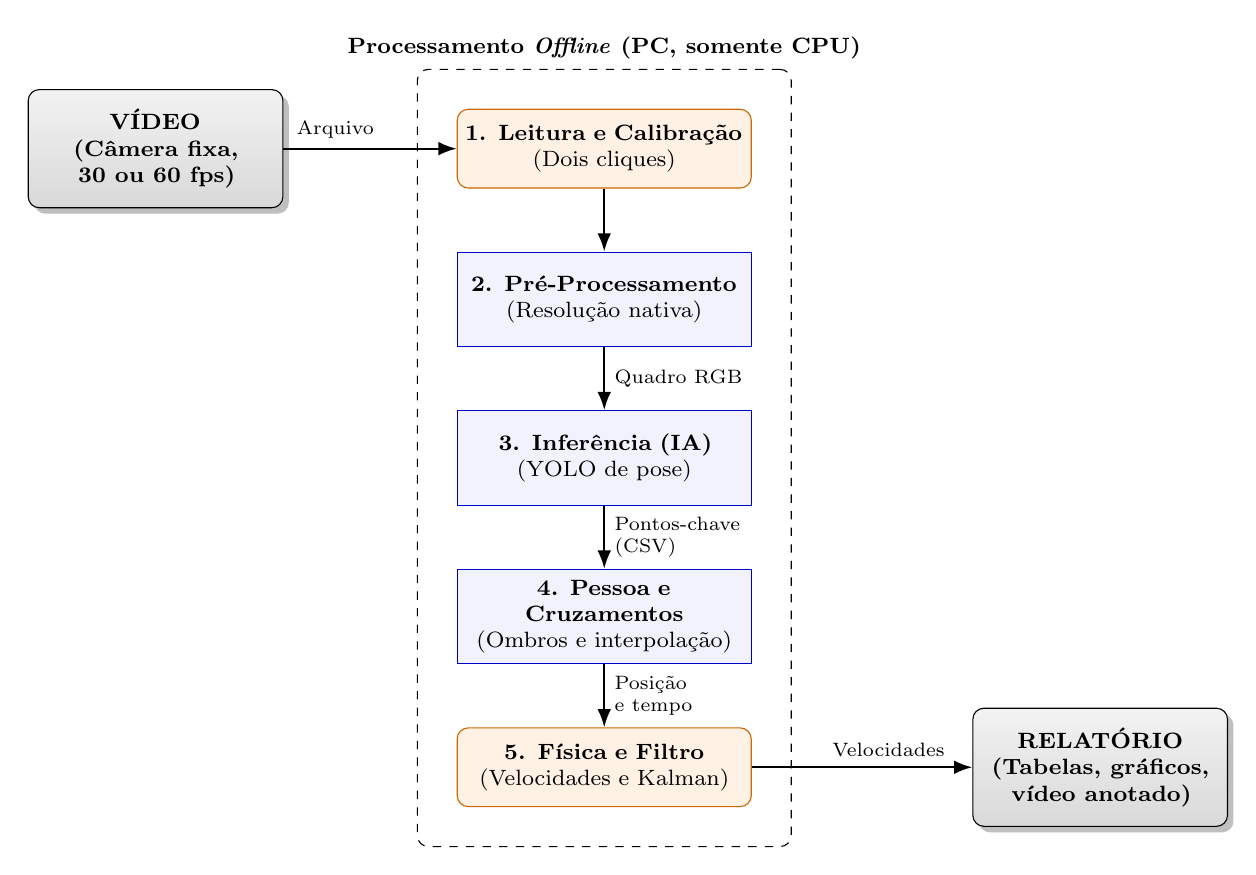
\begin{tikzpicture}[node distance=0.8cm and 1cm, auto]

    % --- NÓS DO DIAGRAMA ---

    % Entrada
    \node [hardware] (cam) {VÍDEO\\(Câmera fixa, 30 ou 60 fps)};

    % Blocos de software
    \node [process, right=2.2cm of cam] (leitura) {\textbf{1. Leitura e Calibração}\\(Dois cliques)};

    \node [software, below=0.8cm of leitura] (preproc) {\textbf{2. Pré-Processamento}\\(Resolução nativa)};

    \node [software, below=0.8cm of preproc] (yolo) {\textbf{3. Inferência (IA)}\\(YOLO de pose)};

    \node [software, below=0.8cm of yolo] (selecao) {\textbf{4. Pessoa e Cruzamentos}\\(Ombros e interpolação)};

    \node [process, below=0.8cm of selecao] (calculo) {\textbf{5. Física e Filtro}\\(Velocidades e Kalman)};

    % Saída
    \node [hardware, right=2.8cm of calculo] (saida) {RELATÓRIO\\(Tabelas, gráficos, vídeo anotado)};

    % Contêiner (caixa tracejada ao redor do software)
    \begin{scope}[on background layer]
        \node [container, fit=(leitura) (preproc) (yolo) (selecao) (calculo), label={[anchor=south, font=\footnotesize]north:\textbf{Processamento \textit{Offline} (PC, somente CPU)}}] (pc) {};
    \end{scope}

    % --- CONEXÕES ---

    \path [line] (cam) -- node[above, pos=0.3, font=\scriptsize] {Arquivo} (leitura);

    \path [line] (leitura) -- (preproc);
    \path [line] (preproc) -- node[right, font=\scriptsize, align=left] {Quadro RGB} (yolo);
    \path [line] (yolo) -- node[right, font=\scriptsize, align=left] {Pontos-chave\\(CSV)} (selecao);
    \path [line] (selecao) -- node[right, font=\scriptsize, align=left] {Posição\\e tempo} (calculo);

    \path [line] (calculo) -- node[above, pos=0.62, font=\scriptsize] {Velocidades} (saida);

\end{tikzpicture}

\fonte{Elaborado pelo autor (2026).}
\label{fig:diagrama_detalhado}
\end{figure}

\subsection{Detalhamento dos Módulos de Software Internos}

O \textit{pipeline} de processamento é constituído por cinco módulos sequenciais. Cada módulo é um programa separado, e os dados brutos ficam gravados entre eles.

\subsubsection{Módulo 1: Leitura do Vídeo e Calibração}
O vídeo é lido quadro a quadro com a biblioteca OpenCV. Como o processamento é \textit{offline}, não há necessidade de leitura assíncrona nem de descarte de quadros: todos os quadros são processados, na ordem. Para cada quadro são registrados dois instantes: o carimbo de tempo informado pelo arquivo, lido logo após a leitura do quadro, e o tempo nominal, calculado como o índice do quadro dividido pela taxa de quadros informada pelo contêiner.

A base de tempo oficial é o carimbo. A análise dos carimbos mostrou que os três vídeos foram gravados a taxa constante, de 30 quadros por segundo no Ensaio A e de 60 nos outros dois. A taxa informada pelo contêiner é uma média, e nos vídeos a 60 quadros por segundo ela é distorcida pelo primeiro intervalo entre quadros, que é anômalo. Por isso o tempo nominal fica no relatório só como referência.
% fonte: diagnostico/Trotando_2.md (seção 1); diagnostico/J_Correndo.md (seção 1); diagnostico/J_Variando.md (seção 1); src/analisar_cruzamentos.py (carregar_keypoints)

A calibração é feita uma vez por vídeo, no primeiro quadro: o usuário clica sobre as duas marcações do solo que delimitam a zona de medição, em uma janela ajustada à tela e com uma lupa em resolução original. A escala resultante é um escalar único $C$, em metros por pixel, dado pela Equação \ref{eq:escala}, com $px_{ref}$ igual à distância em pixels entre as duas marcações.

\subsubsection{Módulo 2: Pré-Processamento Matricial}
As redes neurais convolucionais trabalham com tensores de entrada de dimensões fixas, e a biblioteca redimensiona o quadro conforme o parâmetro de resolução de inferência (\texttt{imgsz}). Neste trabalho, esse parâmetro é a resolução nativa do vídeo, arredondada para o múltiplo de 32 imediatamente superior ao maior lado da imagem, porque as redes da família YOLO reduzem a imagem por um fator de 32: 1920 para os vídeos de 1920$\times$1080 pixels e 1280 para o de 1280$\times$720. A normalização dos valores dos pixels é feita pela própria biblioteca.

Essa escolha decorre de um experimento, descrito na Seção \ref{sec:resultado_imgsz}.

\subsubsection{Módulo 3: Motor de Inferência (YOLO)}
O quadro alimenta a rede YOLO, na variante de estimação de pose de menor tamanho do YOLO26, o modelo \texttt{yolo26n-pose}. Para cada pessoa detectada, o modelo devolve a caixa delimitadora, a confiança da detecção e as coordenadas $(x, y)$ e a confiança de cada um dos 17 pontos-chave. A confiança mínima de detecção foi fixada explicitamente em 0,25. Os pesos são pré-treinados: o treinamento do modelo não faz parte deste trabalho.

A inferência é executada em CPU. O resultado de cada quadro é gravado no arquivo CSV, junto com o índice do quadro, os dois instantes de tempo e o número de pessoas detectadas.

\subsubsection{Módulo 4: Seleção da Pessoa e Detecção dos Cruzamentos}
Em cada quadro com mais de uma pessoa detectada, é escolhida a de maior caixa delimitadora. Dessa pessoa extrai-se o ponto de medição, o centro entre os dois ombros, exigindo confiança mínima de 0,35 em cada ombro. Quadros que não cumprem o critério ficam sem medição e não são preenchidos nem interpolados.

Sobre a série de posições válidas, uma máquina de estados percorre os quadros na ordem. O primeiro cruzamento da zona define a direção da corrida e a linha de entrada, e o cruzamento seguinte define a linha de saída. O instante de cada cruzamento é obtido por interpolação linear entre as duas medições válidas que cercam a linha. O cruzamento interpolado sobre um intervalo superior a 0,25~s é marcado como inválido, mas não é descartado: acima disso, o erro da interpolação linear cresce com o quadrado do intervalo, e as duas medições podem nem pertencer ao mesmo movimento. As equações estão na Seção \ref{sec:estimativa}.
% fonte: src/analisar_cruzamentos.py (GAP_MAX_CRUZAMENTO_S e justificativa)

\subsubsection{Módulo 5: Cálculo Físico e Suavização}
\begin{enumerate}
    \item \textbf{Conversão de Espaço:} aplica-se o fator de calibração linear $C$ para converter a posição em pixels para metros.
    \item \textbf{Velocidade Média no Trecho:} distância entre as marcações dividida pelo tempo entre os dois cruzamentos (Equação \ref{eq:vmedia}).
    \item \textbf{Velocidade Instantânea Bruta:} para cada par de medições válidas consecutivas, o deslocamento projetado na direção da corrida dividido pelo intervalo de tempo. Ela é mantida no relatório sem nenhum filtro.
    \item \textbf{Filtro e Suavizador de Kalman:} calculados ao lado da velocidade bruta, a partir da mesma série de posições (Seção \ref{sec:kalman}).
    \item \textbf{Diagnóstico:} disponibilidade de medição no trecho, maior intervalo sem medição, ruído de posição e quadros rejeitados pelo filtro.
\end{enumerate}

A derivada numérica amplifica o ruído de posição, porque divide a diferença entre duas posições vizinhas por um intervalo curto: com ruído de posição de desvio padrão $\sigma_z$ e taxa de quadros $f$, a velocidade instantânea tem desvio de cerca de $\sqrt{2}\,\sigma_z f$. A 60 quadros por segundo, um ruído de 1~cm já produz cerca de 0,85~m/s.
% cálculo: sqrt(2) × 0,01 m × 60/s = 0,85 m/s

Para conferir cada medição, uma ferramenta de visualização reproduz o vídeo com as linhas da zona de medição, a pessoa selecionada, o ponto medido e um recorte ampliado do atleta, e desenha, ao longo do trecho, a velocidade instantânea bruta e a do suavizador de Kalman. Ao fim da passagem, ela mostra a velocidade média no trecho calculada com o tempo do cronômetro e com o da visão computacional, sem e com o filtro, e a velocidade mínima e a máxima do suavizador no trecho (Figura \ref{fig:tela_variando}). Os números da tela são os mesmos do relatório do programa.

% NOVO
\begin{figure}[H]
\centering
\caption{Tela da ferramenta de visualização ao fim do Ensaio C (velocidade variada, 20~m)}
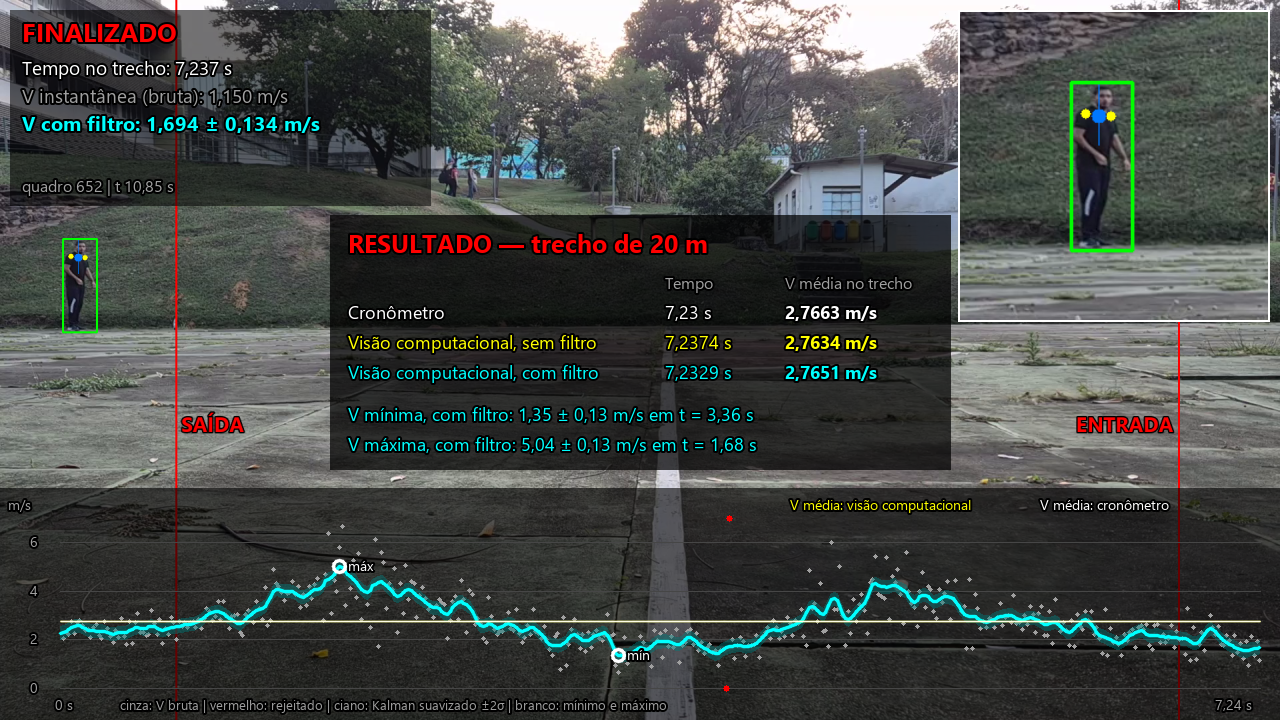
\includegraphics[width=\textwidth]{figuras/tela_J_Variando.png}
\fonte{Elaborado pelo autor (2026), com \texttt{src/visualizar\_medicao.py}.}
\label{fig:tela_variando}
\end{figure}
% fonte: python src/visualizar_medicao.py --video J_Variando --salvar-quadro (quadro 652, o último)

% ----------------------------------------------------------
% SEÇÃO 3.2 - EQUIPAMENTO DE REFERÊNCIA
% ----------------------------------------------------------
\section{Equipamento de Referência}
\label{sec:referencia}

Para a validação do sistema, a referência prevista é um sistema de fotocélulas, a alternativa prática de campo à cronometragem automática (Seção \ref{sec:fotocelulas}). Nos ensaios preliminares apresentados neste trabalho, as fotocélulas ainda não estavam disponíveis, e a referência foi o cronômetro manual (Subseção \ref{sec:cronometro}), de incerteza maior.

\subsection{Aparelho e Posicionamento}
O sistema de fotocélulas da EEFFTO [CONFIRMAR com o coorientador: marca, modelo, feixe único ou duplo, resolução temporal e altura dos feixes] registra o instante em que o atleta interrompe o feixe em cada uma das duas linhas da zona de medição. As fotocélulas são posicionadas sobre as mesmas marcações usadas na calibração do vídeo, de modo que o sistema de visão e a fotocélula medem o mesmo trecho.

\subsection{Lógica de Cálculo e Limitações da Referência}
A fotocélula fornece a velocidade média no trecho, calculada pela Equação \ref{eq:vmedia} com os instantes registrados nas linhas de entrada e de saída, separadas pela distância $D$. Ela não registra variações de velocidade dentro do trecho. Por isso, a comparação é feita com a velocidade média no trecho do sistema, sem e com o filtro.

O erro típico de 0,02~s no feixe duplo e de 0,03~s no feixe único vem de testes repetidos de sprint e inclui a variação do próprio atleta entre tentativas. Quando o sistema e a fotocélula medem a mesma passagem, essa variação não entra, e o erro da fotocélula na comparação é menor que esses valores.
% fonte: Haugen e Buchheit (2016), seções 4.3.1 e 4.3.2 ("reliability data across short-sprint studies")

\subsection{Referência Provisória: Cronômetro Manual}
\label{sec:cronometro}
Nos ensaios preliminares, o tempo de cada corrida na zona de medição foi cronometrado manualmente, e a velocidade de referência foi calculada pela Equação \ref{eq:vmedia}. O tempo manual inclui o tempo de reação de quem opera o cronômetro, e a diferença de 0,19~s entre cronometristas é muito maior que a contribuição do processamento para a incerteza do sistema de visão (Seção \ref{sec:orcamento}), de modo que, com essa referência, a comparação mede principalmente a incerteza do próprio cronômetro. As fotocélulas substituem o cronômetro como referência na validação (Seção \ref{sec:resultado_fotocelula}).

% ----------------------------------------------------------
% SEÇÃO 3.3 - DESENVOLVIMENTO DO PROTÓTIPO
% ----------------------------------------------------------
\section{Desenvolvimento do Protótipo de Visão Computacional}

Esta seção descreve o hardware, o software e os algoritmos do sistema de medição de velocidade, que integra uma câmera fixa e um conjunto de programas de visão computacional executados em computador pessoal, de modo que cada resultado possa ser reproduzido a partir dos dados brutos gravados.

\subsection{Hardware e Montagem}

\subsubsection{Especificações de Processamento}
\begin{itemize}
    \item \textbf{Unidade Central:} Notebook Dell G15 5520, com processador Intel Core i5-12500H, 24~GB de memória RAM e sistema operacional Windows 11. O equipamento tem uma placa de vídeo NVIDIA GeForce RTX 3050, que não foi usada: a versão instalada do PyTorch não tem suporte a GPU, e a inferência da rede neural é feita somente em CPU.
    % fonte: Win32_Processor e Win32_ComputerSystem (lidos em 2026-10-16); resultados/keypoints/*_imgsz*.json (dispositivo cpu, torch 2.14.1+cpu)
\end{itemize}

\subsubsection{Sistema de Captura de Imagem}
\begin{itemize}
    \item \textbf{Dispositivo:} Celular Samsung Galaxy S24, nos três ensaios; o Ensaio A foi gravado com uma configuração de vídeo inferior à dos ensaios de 20~m.
    % fonte: informação do autor (2026-10-16 e 2026-10-17)
    \item \textbf{Formato:} os vídeos dos Ensaios B e C têm 1920$\times$1080 pixels, a 60 quadros por segundo; o do Ensaio A tem 1280$\times$720 pixels, a 30 quadros por segundo. Todos foram gravados a taxa constante (Módulo 1), e a análise é feita sempre sobre o arquivo original da câmera.
    % fonte: resultados/keypoints/*_imgsz*.json; diagnostico/Trotando_2.md
\end{itemize}

\subsubsection{Montagem e Cenário Experimental}
A medição baseia-se no deslocamento do ponto medido em uma vista lateral. A câmera é fixada em tripé, à altura do tronco do atleta, sem movimento de rotação, inclinação ou \textit{zoom} durante a gravação, e a imagem é estável.

\begin{itemize}
    \item \textbf{Posicionamento:} O atleta atravessa o quadro na horizontal, da direita para a esquerda. Foram usadas duas montagens: zona de 20~m, demarcada no solo por duas garrafas brancas, com a câmera a 21~m da linha de corrida (Ensaios B e C); e zona de 5~m, demarcada por dois chinelos pretos, com a câmera a 6~m (Ensaio A).
    % fonte: diagnostico/J_Correndo.md; experimentos/2026-10-17-trotando_2.md; informação do autor (2026-10-17: Ensaio A a 6 m; câmera à altura do tronco nos três)
    \item \textbf{Calibração de Escala:} Para a conversão de coordenadas de imagem em metros, os dois pontos de referência no solo são marcados por dois cliques no primeiro quadro (Módulo 1).
\end{itemize}

\subsection{Ambiente de Software e Bibliotecas}

O software roda em Windows 11, em Python 3.14.7.

Para garantir o isolamento e a reprodutibilidade, o sistema opera em um ambiente virtual (\textit{venv}) com as versões das bibliotecas fixadas. A fixação é necessária porque os mesmos pesos, no mesmo vídeo, produziram resultados diferentes em duas versões da biblioteca de inferência: com a resolução de inferência de 640 pixels, a versão 8.4.133 detectou o corredor em 89 quadros do vídeo, e a 8.4.174, em 134 quadros, por causa de confianças de detecção ligeiramente maiores na versão mais nova, sobre um limiar de 0,25. Por isso, cada extração grava as versões utilizadas e o resumo (\textit{hash}) dos pesos em um arquivo ao lado do CSV.
% fonte: diagnostico/J_Correndo.md (seção 3)

As bibliotecas usadas são:

\begin{enumerate}
    \item \textbf{OpenCV (\texttt{opencv-python}, versão 5.0.0):} Leitura dos quadros e dos carimbos de tempo do vídeo e interface gráfica da calibração e da visualização.

    \item \textbf{Ultralytics YOLO (\texttt{ultralytics}, versão 8.4.174):} Framework responsável pela implementação do modelo de detecção e estimação de pose. Utiliza-se o modelo \texttt{yolo26n-pose}, de pesos pré-treinados\footnote{É importante distinguir as etapas do ciclo de vida de \textit{Machine Learning}: o \textit{treinamento} da rede neural, etapa computacionalmente intensiva, é realizado previamente pelo fornecedor do modelo. Este trabalho executa apenas a \textit{inferência} (utilização do modelo já treinado).}. Esta biblioteca retorna as caixas delimitadoras, as confianças e as coordenadas dos pontos-chave de cada pessoa detectada.

    \item \textbf{NumPy (\texttt{numpy}, versão 2.5.3):} Biblioteca de computação numérica em Python, empregada nos cálculos vetoriais e na implementação do filtro e do suavizador de Kalman e da busca de parâmetros.

    \item \textbf{PyTorch (\texttt{torch}, versão 2.14.1, em CPU):} Atua como \textit{backend} de tensores para a execução da rede neural.
\end{enumerate}
% fonte: resultados/keypoints/J_Correndo_imgsz1920.json (versoes)

% ----------------------------------------------------------
% SEÇÃO 3.3.3 - ALGORITMO DE DETECÇÃO (YOLO)
% ----------------------------------------------------------
\subsection{Algoritmo de Detecção (YOLO)}

O algoritmo de detecção adotado fundamenta-se na arquitetura YOLO, que modela a detecção como um problema de regressão único. Foi utilizado o modelo \texttt{yolo26n-pose}, o menor da família, inicialmente escolhido por velocidade de processamento. Como a medição é \textit{offline}, o ganho de velocidade não é necessário, e a avaliação de modelos maiores fica como trabalho futuro (Seção \ref{sec:trabalhos_futuros}).
% fonte: README.md (pendências: modelos YOLO maiores)

\subsubsection{Funcionamento da Rede Neural}
O funcionamento geral da arquitetura está descrito na Seção \ref{sec:visao}. A variante de pose prediz, além da caixa delimitadora, as coordenadas $(x, y)$ e a confiança de cada um dos 17 pontos-chave do corpo; este trabalho usa apenas os dois ombros (pontos 5 e 6). O modelo detecta uma única classe, pessoa: os pesos usados têm somente a classe \textit{person}. A escolha, entre as pessoas detectadas, daquela que é o atleta é feita por regra própria (Subseção \ref{sec:selecao}).
% fonte: yolo26n-pose.pt (model.names = {0: 'person'}), verificado em 2026-10-16

\subsubsection{Pós-Processamento: Supressão Não-Máxima (NMS)}
A saída bruta de um detector frequentemente gera múltiplas caixas redundantes para um único atleta. Nas arquiteturas que utilizam a supressão não-máxima (NMS, do inglês \textit{non-maximum suppression}), seleciona-se a caixa com o maior grau de confiança e descartam-se as demais candidatas que apresentam uma IoU superior a um limiar pré-definido. O YOLO26 tem duas saídas: uma de ponta a ponta, que dispensa a NMS, e uma convencional, seguida de NMS \cite{jocher2026yolo26}. Com a versão da biblioteca usada (\texttt{ultralytics} 8.4.174) e os argumentos padrão, a inferência deste trabalho usa o modo convencional, com NMS e limiar de IoU de 0,7.
% fonte: ultralytics/cfg/default.yaml (iou: 0.7; nms: None = NMS externo) e ultralytics/cfg/models/26/yolo26-pose.yaml; inferência de teste em 2026-10-16 (non_max_suppression chamada com end2end=False)

% ----------------------------------------------------------
% SEÇÃO 3.3.4 - ALGORITMO DE ESTIMATIVA DE VELOCIDADE
% ----------------------------------------------------------
\subsection{Algoritmo de Estimativa de Velocidade}
\label{sec:estimativa}

Este módulo converte os dados brutos de detecção em grandezas cinemáticas. Há dois estimadores. O principal é a \textbf{velocidade média no trecho}, obtida pelos instantes em que o ponto medido cruza duas linhas do solo separadas por uma distância conhecida: reproduz, em software, o princípio da fotocélula (Equação \ref{eq:vmedia}). O segundo é a \textbf{velocidade instantânea}, baseada no deslocamento de pixels com fator de calibração, adaptado do método LV-YOLO, originalmente proposto para veículos.

\subsubsection{Associação Temporal e Rastreamento}
\label{sec:selecao}
Este trabalho não utiliza algoritmo de rastreamento de objetos, como o SORT. Em cada quadro, quando há mais de uma pessoa detectada, o atleta é a de maior caixa delimitadora. Os quadros não são associados entre si: o cálculo usa a posição de cada quadro com medição válida, e um quadro sem medição não é preenchido, de modo que o intervalo de tempo do par seguinte simplesmente cresce.

A regra tem uma fragilidade conhecida: quando outra pessoa ou um objeto ao fundo é detectado com caixa maior que a do corredor, a regra o escolhe no lugar do atleta. Isso aconteceu uma vez, no quadro 279 do Ensaio C (Seção \ref{sec:resultado_ensaios}). Escolher a detecção mais próxima da posição anterior do atleta (continuidade de trajetória) é uma correção possível, que não foi aplicada e fica como trabalho futuro. O teste de inovação do filtro de Kalman rejeita esse tipo de erro.
% fonte: diagnostico/J_Variando.md (seção 4); README.md (pendências)

\subsubsection{Definição do Ponto de Medição}
O corpo humano é um sistema articulado: o centro da caixa delimitadora oscila com o movimento dos braços e das pernas. O ponto de referência adotado é o \textbf{centro entre os dois ombros}, obtido a partir dos pontos-chave 5 e 6 e aceito apenas quando os dois ombros têm confiança mínima de 0,35.

A escolha foi comparada, nos três ensaios, com outros pontos do corpo, pelo critério de menor ruído de posição (Seção \ref{sec:resultado_ponto}).

O ponto medido oscila horizontalmente com a rotação do tronco e o balanço dos braços, em frequência ligada à cadência da corrida. Essa oscilação é movimento real do ponto medido, não erro de medição, mas o ponto medido não é o centro de massa do atleta. Portanto, o sistema estima a velocidade horizontal aparente do ponto médio entre os ombros, projetada no plano de calibração.

\subsubsection{Modelo Matemático}
O cálculo segue as etapas abaixo.

\textbf{1. Fator de Calibração ($C$):}
A transformação do espaço de imagem para o espaço métrico é feita pelo fator $C$ [$metros/pixel$] da Equação \ref{eq:escala}, com $px_{ref} = x_{max} - x_{min}$, em que $x_{min}$ e $x_{max}$ são as abscissas das duas marcações, separadas pela distância real $D$.

\textbf{2. Instante de cruzamento por interpolação linear:}
Se $x_0$ e $x_1$ são as posições (em pixels) das duas medições válidas consecutivas que cercam uma linha de abscissa $x_L$, nos instantes $t_0$ e $t_1$, o instante do cruzamento é
\begin{equation} \label{eq:alfa}
    \alpha = \frac{x_L - x_0}{x_1 - x_0}, \qquad t_{cruz} = t_0 + \alpha\,(t_1 - t_0),
\end{equation}
aceito apenas se $0 \le \alpha \le 1$.

\textbf{3. Velocidade Média no Trecho ($\bar{v}$):}
Pela Equação \ref{eq:vmedia}, com os instantes de entrada e saída, $t_{ent}$ e $t_{sai}$, interpolados pela Equação \ref{eq:alfa}.

\textbf{4. Velocidade Instantânea ($V_{inst}$):}
Para dois quadros com medição válida $i-1$ e $i$, com $s = +1$ se a corrida é no sentido de $x$ crescente e $s = -1$ no sentido contrário:
\begin{equation} \label{eq:vinst}
    V_{inst,i} = s\,\frac{(x_i - x_{i-1})\,C}{t_i - t_{i-1}} \quad [m/s]
\end{equation}
O sinal é mantido: um valor negativo indica deslocamento contrário ao sentido da corrida, e é contado e reportado, não descartado. O deslocamento não é tomado em módulo, porque o módulo transformaria o ruído de posição, que é simétrico, em um viés sempre positivo.
% fonte: src/analisar_cruzamentos.py (calcular_velocidades_instantaneas)

\subsubsection{Filtro e Suavizador de Kalman}
\label{sec:kalman}
A velocidade instantânea bruta (Equação \ref{eq:vinst}) é mantida no relatório sem nenhum filtro: não é aplicada média móvel nem média exponencial sobre os números reportados. Ao lado dela, a posição medida passa por um filtro e por um suavizador de Kalman, cujas equações seguem \citeonline{sarkka2023bayesian}: o modelo de movimento e a matriz $\mathbf{Q}$ vêm do Exemplo 4.5; o filtro, do Teorema 6.6; o suavizador, do Teorema 12.2; e a verossimilhança calculada pelas inovações, do Teorema 16.9. O filtro combina, a cada quadro, a previsão feita por um modelo de movimento com a nova medição, pesando cada uma pela sua incerteza. O suavizador, possível porque o processamento é \textit{offline}, revisa depois cada estimativa usando também as medições posteriores a ela. Para um modelo linear com ruídos gaussianos, o resultado é a média da distribuição do estado dadas as medições, que é a estimativa de menor erro quadrático médio. Os passos são descritos a seguir, e a Tabela \ref{tab:grandezas} reúne as grandezas e a origem de cada uma.

\textbf{Estado e modelo de movimento.} O estado do filtro é $\mathbf{x}_k = [p_k,\ v_k]^T$, com $p$ a posição (m) do ponto medido, projetada na direção da corrida, e $v$ a sua velocidade (m/s). O modelo é o de velocidade quase constante: a velocidade não é suposta constante, mas a sua variação, isto é, a aceleração, é tratada como um ruído aleatório branco de intensidade $q$ [m$^2$/s$^3$]. Integrando esse ruído durante o intervalo $\Delta t_k$ entre dois quadros, obtém-se:
\begin{equation} \label{eq:kalman_modelo}
    \mathbf{x}_k = \mathbf{F}_k\,\mathbf{x}_{k-1} + \mathbf{w}_k, \qquad
    \mathbf{F}_k = \begin{bmatrix} 1 & \Delta t_k \\ 0 & 1 \end{bmatrix}, \qquad
    \mathbf{Q}_k = q \begin{bmatrix} \Delta t_k^3/3 & \Delta t_k^2/2 \\ \Delta t_k^2/2 & \Delta t_k \end{bmatrix}
\end{equation}
em que $\mathbf{w}_k$ é o ruído de processo, de média zero e covariância $\mathbf{Q}_k$. A matriz $\mathbf{F}_k$ diz que a nova posição é a anterior mais a velocidade vezes o intervalo, e que a velocidade se mantém; $\mathbf{Q}_k$ diz quanto a posição e a velocidade podem mudar por causa da aceleração que o modelo não representa. Na prática, $\sqrt{q\,\Delta t}$ é a variação típica da velocidade de um quadro para o outro: com o $q$ do Ensaio B (2,75~m$^2$/s$^3$) e $\Delta t = 1/60$~s, 0,21~m/s.
% fonte: diagnostico/kalman_caracterizacao.md (seção 1)

\textbf{Medição.} A medição é a posição dos ombros, convertida para metros e projetada na direção da corrida:
\begin{equation} \label{eq:kalman_medicao}
    z_k = \mathbf{H}\,\mathbf{x}_k + \nu_k, \qquad \mathbf{H} = [1\ \ 0], \qquad \nu_k \sim \mathcal{N}(0, R)
\end{equation}
A variância $R$ do ruído de medição parte do ruído do ponto medido, $\sigma_x$, estimado pela segunda diferença da posição $x_k$ em pixels. Em três quadros consecutivos, a combinação $x_{k+1} - 2x_k + x_{k-1}$ cancela o movimento uniforme e deixa só o ruído, com desvio padrão $\sqrt{6}\,\sigma_x$. Para que valores absurdos, como o do quadro 279, não distorçam a estimativa, o desvio é calculado pela mediana dos desvios absolutos, multiplicada por 1,4826, fator que a torna igual ao desvio padrão para dados gaussianos:
\begin{equation} \label{eq:sigma_x}
    d_k = x_{k+1} - 2x_k + x_{k-1}, \qquad
    \sigma_x = \frac{1{,}4826 \cdot \operatorname{mediana}\left(\left|d_k - \operatorname{mediana}(d)\right|\right)}{\sqrt{6}}
\end{equation}
Como a segunda diferença inclui também a parte do movimento real que não é uniforme em três quadros, $\sigma_x$ é um limite superior para o ruído do ponto. A variância de medição é
\begin{equation} \label{eq:kalman_r}
    R = (\kappa\,\sigma_x\,C)^2
\end{equation}
em que $C$ é o fator de calibração (Equação \ref{eq:escala}) e $\kappa$ é um fator escolhido por máxima verossimilhança, junto com $q$ (parágrafo Sintonia, abaixo). A raiz de $R$, $\sigma_z = \kappa\,\sigma_x\,C$, é o desvio padrão do ruído de medição, em metros.
% fonte: src/analisar_cruzamentos.py (ruido_segunda_diferenca; aplicar_kalman, sigma_z_px)

\textbf{Início.} O filtro começa na primeira medição válida: a posição inicial é essa medição, com variância $R$, e a velocidade inicial é zero, com desvio padrão de 10~m/s, valor grande que equivale a dizer que a velocidade é desconhecida. As duas primeiras medições servem para fixar o estado e não entram no cálculo da verossimilhança.
% fonte: src/kalman.py (DP_INICIAL_VELOCIDADE, ModeloCV.p0, filtrar)

\textbf{Predição.} A cada quadro, a estimativa do estado e a sua matriz de covariância $\mathbf{P}$ são levadas adiante pelo modelo:
\begin{equation} \label{eq:kalman_predicao}
    \hat{\mathbf{x}}_k^- = \mathbf{F}_k\,\hat{\mathbf{x}}_{k-1}, \qquad
    \mathbf{P}_k^- = \mathbf{F}_k\,\mathbf{P}_{k-1}\,\mathbf{F}_k^T + \mathbf{Q}_k
\end{equation}
O passo de tempo $\Delta t_k$ é variável: um quadro sem medição válida vira apenas predição, e o intervalo até a medição seguinte simplesmente cresce, sem interpolação nem preenchimento.

\textbf{Inovação.} A inovação $e_k$ é a diferença entre a medição e a sua previsão, e $S_k$ é a variância esperada dessa diferença, que soma a incerteza da previsão e a da medição:
\begin{equation} \label{eq:kalman_inovacao}
    e_k = z_k - \mathbf{H}\,\hat{\mathbf{x}}_k^-, \qquad
    S_k = \mathbf{H}\,\mathbf{P}_k^-\,\mathbf{H}^T + R
\end{equation}

\textbf{Ganho de Kalman.} O ganho define quanto da inovação é incorporado ao estado:
\begin{equation} \label{eq:kalman_ganho}
    \mathbf{K}_k = \frac{\mathbf{P}_k^-\,\mathbf{H}^T}{S_k}
    = \begin{bmatrix} P^-_{11}/S_k \\ P^-_{21}/S_k \end{bmatrix}
\end{equation}
O ganho é a razão entre a incerteza da previsão e a incerteza total. A sua componente de posição fica entre 0 e 1: perto de 0, o filtro confia na previsão e quase ignora a medição; perto de 1, adota a medição. A componente de velocidade, em s$^{-1}$, diz quanto a velocidade estimada muda por metro de inovação. Na segunda medição, como a velocidade ainda é desconhecida, o ganho de posição é praticamente 1 e o de velocidade é igual à taxa de quadros: o filtro aceita a medição inteira, e a velocidade passa a ser a diferença entre as duas primeiras posições dividida pelo intervalo. A incerteza diminui a cada medição, e por volta da décima o ganho atinge o valor de regime (Tabela \ref{tab:ganho}).

\textbf{Atualização.} A estimativa e a covariância são corrigidas por:
\begin{equation} \label{eq:kalman_atualizacao}
    \hat{\mathbf{x}}_k = \hat{\mathbf{x}}_k^- + \mathbf{K}_k\,e_k, \qquad
    \mathbf{P}_k = (\mathbf{I} - \mathbf{K}_k\mathbf{H})\,\mathbf{P}_k^-\,(\mathbf{I} - \mathbf{K}_k\mathbf{H})^T + \mathbf{K}_k\,R\,\mathbf{K}_k^T
\end{equation}
A forma usada para $\mathbf{P}_k$ é algebricamente igual a $\mathbf{P}_k^- - \mathbf{K}_k S_k \mathbf{K}_k^T$, a forma usual, mas mantém a matriz simétrica e positiva mesmo com erros de arredondamento.

\textbf{Teste de inovação e o limite de 5 desvios padrão.} Se o modelo descreve bem os dados, a inovação tem distribuição normal de média zero e variância $S_k$. A inovação normalizada, $e_k/\sqrt{S_k}$, é então normal padrão, e o seu quadrado, chamado NIS (do inglês \textit{normalized innovation squared}),
\begin{equation} \label{eq:nis}
    \mathrm{NIS}_k = \frac{e_k^2}{S_k}
\end{equation}
segue a distribuição qui-quadrado com um grau de liberdade: tem média 1, e 95\% dos seus valores ficam abaixo de 3,84. Uma medição com $\mathrm{NIS}_k > 25$, isto é, com inovação maior que 5 desvios padrão, é rejeitada: o quadro vira apenas predição e é listado no relatório.

O teste existe para rejeitar erros de identidade, isto é, a detecção de outra pessoa ou objeto no lugar do atleta, e não ruído nem movimento real. O limite de 5 desvios padrão foi escolhido pelos seguintes motivos (Tabela \ref{tab:inovacao}):
\begin{itemize}
    \item o erro de identidade observado, no quadro 279 do Ensaio C, foi uma inovação de 8,5~m, ou 757 desvios padrão: qualquer limite razoável o rejeita;
    \item a maior inovação de uma medição boa foi de 4,2 desvios padrão (quadro 317 do Ensaio C, um surto real de velocidade dentro da passada), e de 3,9 e 2,9 nos outros dois ensaios: o limite precisa ficar acima disso para não descartar movimento real;
    \item se o erro de medição fosse exatamente gaussiano, a chance de uma medição boa passar de 5 desvios padrão seria de $5{,}7 \times 10^{-7}$, ou 0,0003 rejeições esperadas nas 493 medições do Ensaio C que passam pelo teste. Com o limite usual de 3 desvios padrão seriam 1,3, mas o filtro rejeitou 9, cinco delas no surto real, porque o erro real tem mais valores grandes do que a distribuição gaussiana prevê;
    \item entre 4 e 10 desvios padrão o resultado não muda: só o quadro 279 é rejeitado, e a velocidade média varia menos de 0,01\% (Tabela \ref{tab:sensibilidade}); 5 desvios padrão fica no meio desse intervalo.
\end{itemize}
Esse limite foi escolhido depois de ver os dados dos dois ensaios de 20~m (Seção \ref{sec:resultado_kalman}). O Ensaio A, que não participou da escolha, serviu de verificação (Seção \ref{sec:resultado_trotando}).
% fonte: diagnostico/kalman_caracterizacao.md (seção 3); experimentos/2026-10-07-kalman.md (seção 8)

\textbf{Sintonia de $q$ e $R$ por máxima verossimilhança.} Os valores de $q$ e de $\kappa$ são os que tornam as inovações observadas mais prováveis. Como cada inovação é gaussiana, com variância $S_k$, o logaritmo da verossimilhança é:
\begin{equation} \label{eq:kalman_verossimilhanca}
    \ln L(q, \kappa) = -\frac{1}{2} \sum_k \left[ \ln(2\pi S_k) + \min(\mathrm{NIS}_k,\ 25) \right]
\end{equation}
Um $q$ pequeno demais faz o filtro reagir devagar às mudanças reais de velocidade, e as inovações ficam grandes; um $q$ grande demais faz o filtro seguir o ruído, e $S_k$ cresce. O máximo de $\ln L$ equilibra os dois efeitos. A busca é feita em grade: $\kappa$ de 0,5 a 6,3, em passos de 12\%, e $q$ de 0,01 a 10\,000~m$^2$/s$^3$, em passos de 26\%, refinados depois em passos de 5\%. Uma medição rejeitada entra na soma com o NIS limitado a 25, para que rejeitar uma medição não aumente artificialmente a verossimilhança.
% fonte: src/kalman.py (GRADE_FATOR_R, GRADE_Q_CV, ajustar, ajustar_r, filtrar)

\textbf{Suavizador.} Depois do filtro, o suavizador percorre a série de trás para a frente:
\begin{equation} \label{eq:kalman_suavizador}
\begin{aligned}
    \mathbf{G}_k &= \mathbf{P}_k\,\mathbf{F}_{k+1}^T\,\left(\mathbf{P}_{k+1}^-\right)^{-1}, \\
    \hat{\mathbf{x}}_k^s &= \hat{\mathbf{x}}_k + \mathbf{G}_k\left(\hat{\mathbf{x}}_{k+1}^s - \hat{\mathbf{x}}_{k+1}^-\right), \\
    \mathbf{P}_k^s &= \mathbf{P}_k + \mathbf{G}_k\left(\mathbf{P}_{k+1}^s - \mathbf{P}_{k+1}^-\right)\mathbf{G}_k^T
\end{aligned}
\end{equation}
O ganho do suavizador, $\mathbf{G}_k$, diz quanto da correção descoberta no instante seguinte, com as medições posteriores, volta para o instante $k$. O suavizador elimina o atraso do filtro, que só usa medições passadas, e reduz a incerteza (Tabela \ref{tab:ganho}).

\textbf{Velocidade média com filtro e faixa de confiança.} Com a posição suavizada, a velocidade média no trecho é recalculada pelos instantes em que ela cruza as duas linhas, interpolados entre quadros: é a velocidade média com filtro, $\bar{v}_K$. A raiz do elemento de velocidade de $\mathbf{P}_k^s$ é o desvio padrão da velocidade suavizada; a faixa de $\pm 2$ desvios padrão corresponde a cerca de 95\% de confiança se o modelo estiver correto.

\textbf{Consistência.} A adequação do filtro aos dados é verificada pelas inovações das medições aceitas. O NIS médio deve ficar perto de 1, cerca de 5\% dos valores devem passar de 3,84, e a inovação normalizada de um quadro não deve se parecer com a do quadro seguinte: a autocorrelação entre quadros consecutivos deve ficar dentro de $\pm 2/\sqrt{n}$, em que $n$ é o número de medições. Como $q$ e $R$ são escolhidos nos mesmos dados, o NIS médio perto de 1 é, em parte, consequência do ajuste; as verificações independentes são o teste com dados sintéticos (Seção \ref{sec:resultado_sintetico}) e o Ensaio A.

% NOVO
\begin{table}[H]
\centering
\footnotesize
\caption{Grandezas do filtro e do suavizador de Kalman}
\label{tab:grandezas}
\begin{tabular}{L{0.12\textwidth}L{0.48\textwidth}L{0.28\textwidth}}
\hline
\textbf{Símbolo} & \textbf{Significado} & \textbf{Origem} \\
\hline
$p$, $v$ & Posição (m) e velocidade (m/s) do ponto medido, na direção da corrida & Estado do filtro \\
$\Delta t_k$ & Intervalo entre medições: 1/30 ou 1/60~s, maior se faltar medição & Carimbos dos quadros \\
$q$ & Intensidade da aceleração aleatória & Máxima verossimilhança \\
$\mathbf{F}_k$, $\mathbf{Q}_k$ & Transição do estado e covariância do ruído de processo & Equação \ref{eq:kalman_modelo} \\
$\mathbf{H}$ & Seleção da posição no estado, $[1\ \ 0]$ & Equação \ref{eq:kalman_medicao} \\
$\sigma_x$ & Ruído do ponto medido, em pixels & Equação \ref{eq:sigma_x} \\
$\kappa$ & Fator sobre $\sigma_x$ & Máxima verossimilhança \\
$C$ & Fator de calibração & Equação \ref{eq:escala} \\
$R$, $\sigma_z$ & Variância e desvio padrão do ruído de medição, em metros & Equação \ref{eq:kalman_r} \\
$e_k$, $S_k$ & Inovação e a sua variância esperada & Equação \ref{eq:kalman_inovacao} \\
$\mathbf{K}_k$ & Ganho de Kalman (posição; velocidade) & Equação \ref{eq:kalman_ganho} \\
NIS & Inovação normalizada ao quadrado: média esperada 1, 95\% abaixo de 3,84 & Equação \ref{eq:nis} \\
25 & Limite do teste de inovação, 5 desvios padrão & Tabela \ref{tab:sensibilidade} \\
$\mathbf{G}_k$ & Ganho do suavizador & Equação \ref{eq:kalman_suavizador} \\
$\pm 2\sigma$ & Faixa de confiança da velocidade: raiz do elemento de velocidade de $\mathbf{P}_k^s$ & Suavizador \\
\hline
\end{tabular}
\fonte{Elaborado pelo autor (2026).}
\end{table}

% ----------------------------------------------------------
% SEÇÃO 3.4 - PROTOCOLO EXPERIMENTAL DE VALIDAÇÃO
% ----------------------------------------------------------
\section{Protocolo Experimental de Validação}
\label{sec:protocolo}

Foram analisados três ensaios preliminares, com o mesmo corredor:
\begin{itemize}
    \item \textbf{Ensaio A} (arquivo \texttt{Trotando\_2}): a primeira gravação do trabalho (29/08/2026), em trote, com zona de 5~m entre dois chinelos pretos e vídeo de 1280$\times$720 pixels a 30 quadros por segundo;
    \item \textbf{Ensaio B} (arquivo \texttt{J\_Correndo}): o atleta parte parado e acelera ao longo da zona de 20~m, com vídeo de 1920$\times$1080 pixels a 60 quadros por segundo;
    \item \textbf{Ensaio C} (arquivo \texttt{J\_Variando}): mesma montagem do anterior, com o atleta variando a velocidade de propósito dentro da zona, para verificar se o sistema acompanha mudanças reais de velocidade.
\end{itemize}
% fonte: experimentos/2026-10-17-trotando_2.md; diagnostico/J_Correndo.md; diagnostico/J_Variando.md; experimentos/2026-10-07-kalman.md
Em todos, a câmera fica em vista lateral, e o corredor atravessa o quadro da direita para a esquerda. Os ensaios de 20~m foram gravados na Escola de Educação Física, Fisioterapia e Terapia Ocupacional (EEFFTO) da UFMG [CONFIRMAR: local exato e data da gravação original no S24], e o Ensaio A, em uma rua residencial. Todos os ensaios são registrados em uma planilha, inclusive os ruins; um ensaio descartado permanece na planilha, com o motivo do descarte.
% fonte: informação do autor (2026-10-16 e 2026-10-17); resultados/ensaios.csv

% NOVO
\subsection{Sessão de Validação com Fotocélulas}
\label{sec:sessao_fotocelulas}
A validação final compara o sistema com as fotocélulas em uma sessão própria [CONFIRMAR: data, local, número de passagens e faixa de velocidades]. As fotocélulas são posicionadas sobre as duas marcações da zona de medição, e a câmera grava as mesmas passagens, de modo que cada passagem é medida pelos dois sistemas.

\section{Validação}
\label{sec:validacao}

Os ensaios preliminares são comparados com o cronômetro: diferença do tempo e da velocidade média no trecho, em valor absoluto e em porcentagem, sem e com o filtro. Também são relatados a disponibilidade de medição no trecho, o maior intervalo sem medição e o ruído de posição.
% fonte: README.md (analisar); resultados/ensaios.csv

Na sessão com fotocélulas, para cada passagem calcula-se a diferença percentual entre a velocidade do sistema e a da fotocélula. Dessas diferenças saem dois números: a diferença média, que indica se o sistema tende a medir para mais ou para menos, e o desvio padrão das diferenças, que mede o erro aleatório do sistema em relação à fotocélula e faz o papel do erro típico definido na Seção \ref{sec:criterios}. O sistema é considerado útil se esse erro for menor ou igual à menor mudança relevante, de cerca de 1\%. Esse desvio inclui também o erro da própria fotocélula.

O filtro de Kalman foi testado antes da aplicação aos vídeos com dados sintéticos de verdade conhecida: 7~s a 60 quadros por segundo, com aceleração e desaceleração, oscilação da passada de 1,3~cm a 3,5~Hz, ruído de medição de 0,77~cm, 10\% de quadros sem medição, uma lacuna de 15 quadros e um erro de identidade de 8~m. Os critérios de aceitação foram escritos antes de rodar a versão final do teste; o resultado está na Seção \ref{sec:resultado_sintetico}.
% fonte: src/validar_kalman.py; experimentos/2026-10-07-kalman.md (seção 7.1)

% ----------------------------------------------------------
% CAPÍTULO 4 - RESULTADOS
% ----------------------------------------------------------
\chapter{RESULTADOS}

Este capítulo apresenta os resultados dos três ensaios preliminares e dos experimentos feitos sobre o método. A referência dos ensaios preliminares é o cronômetro manual (Subseção \ref{sec:cronometro}), e por isso o capítulo descreve principalmente as contribuições do processamento para a incerteza, e não a exatidão do sistema. A comparação com as fotocélulas está na Seção \ref{sec:resultado_fotocelula}. Os dados, os programas e os registros que geram cada tabela e figura estão no repositório descrito no Apêndice \ref{ap:repositorio}.

% ----------------------------------------------------------
% SEÇÃO 4.1 - RESOLUÇÃO DE ENTRADA DO DETECTOR
% ----------------------------------------------------------
\section{Resolução de Entrada do Detector}
\label{sec:resultado_imgsz}

O Ensaio B foi inicialmente processado com a resolução de inferência padrão da biblioteca (640 pixels). O corredor, com cerca de 137 pixels de altura no vídeo, chegava ao modelo com cerca de 46 pixels e foi detectado em apenas 30\% dos quadros em que atravessava o campo de visão. Isso motivou um experimento que variou apenas a resolução de inferência (640, 1280 e 1920 pixels), mantidos fixos o modelo, o limiar de detecção, a regra de seleção da pessoa, a calibração e o ambiente de software.
% fonte: experimentos/2026-10-07-imgsz-J_Correndo.md (seções 1 a 3 e 9); diagnostico/J_Correndo.md (seção 2)

A hipótese era que aumentar a resolução aumentaria a disponibilidade de medição válida dos ombros no trecho de 20~m. O experimento seria considerado desfavorável se a disponibilidade não subisse pelo menos 10 pontos percentuais, se outra pessoa fosse selecionada no lugar do corredor ou se o ruído do ponto medido aumentasse. Esses critérios foram escritos antes de rodar as variantes de 1280 e 1920 pixels, mas depois de se observar a variante de 640 pixels, que motivou o experimento.

A Tabela \ref{tab:imgsz} usa duas métricas diferentes. A \textbf{detecção} é a fração dos quadros da passagem pelo campo de visão em que o corredor foi detectado. A \textbf{disponibilidade} é a fração dos quadros entre os dois cruzamentos com medição válida dos dois ombros, com confiança mínima de 0,35 em cada um.

\begin{table}[H]
\centering
\small
\caption{Efeito da resolução de inferência no Ensaio B}
\label{tab:imgsz}
\begin{tabular}{L{0.42\textwidth}ccc}
\hline
 & \textbf{640 px} & \textbf{1280 px} & \textbf{1920 px (nativa)} \\
\hline
Altura do corredor na entrada do modelo (px) & $\approx 46$ & $\approx 91$ & $\approx 137$ \\
Quadros com pessoa detectada (de 807) & 134 & 558 & 693 \\
Detecção do corredor durante a passagem & 30\% & 100\% & 100\% \\
Disponibilidade de medição no trecho & 13,4\% & 100\% & 100\% \\
Intervalo de interpolação na entrada (ms) & 233 & 17 & 17 \\
Intervalo de interpolação na saída (ms) & 3149 & 17 & 17 \\
Ruído do ponto medido, $\sigma_x$ (px) & 1,46 & 0,82 & 0,58 \\
Processamento (ms por quadro, CPU) & 65 & 145 & 292 \\
Tempo no trecho (s) & 4,1488 & 3,4013 & 3,4090 \\
Velocidade média no trecho (m/s) & 4,8207 & 5,8801 & 5,8669 \\
Diferença para o cronômetro & $-16{,}1\%$ & $+2{,}31\%$ & $+2{,}08\%$ \\
Situação (intervalo $\le$ 0,25~s) & inválido & válido & válido \\
\hline
\end{tabular}
\fonte{Elaborado pelo autor (2026).}
\end{table}
% fonte: experimentos/2026-10-07-imgsz-J_Correndo.md (tabelas das seções 4, 8 e 9)

Com 640 pixels, o cruzamento da linha de saída ficou sem medição válida próxima, e a interpolação atravessou 3,15~s, misturando a corrida com a pessoa caminhando de volta, o que produziu uma diferença de $-16{,}1\%$ para o cronômetro. Com 1280 ou 1920 pixels, a disponibilidade no trecho foi de 100\%, e os dois cruzamentos foram interpolados entre quadros consecutivos (17~ms). Nenhum critério desfavorável foi atingido: a disponibilidade subiu 87 pontos percentuais, o corredor foi sempre a pessoa selecionada no trecho, e o ruído do ponto medido diminuiu.

Entre 1280 e 1920 pixels não há diferença nas métricas primárias; o tempo do trecho difere em 7,7~ms (0,23\%). A diferença está no ruído do ponto medido (0,58 contra 0,82 pixel). Foi adotada a resolução nativa do vídeo, por empatar na métrica primária, ter menor ruído e ser coerente com o processamento \textit{offline}. O custo é de cerca de 4 minutos de CPU por vídeo.
% fonte: experimentos/2026-10-07-imgsz-J_Correndo.md (seções 5 e 9)

O mesmo efeito foi verificado depois no Ensaio A, com 640 e 1280 pixels, a resolução nativa desse vídeo. Ali o corredor tinha cerca de 294 pixels de altura no vídeo e chegava ao modelo com cerca de 148 pixels mesmo a 640, e foi detectado em todo o trecho nas duas resoluções. A resolução nativa reduziu o ruído do ponto medido de 1,44 para 1,02 pixel (29\%) e mudou a velocidade média em 0,74\%. O efeito da resolução depende, portanto, do tamanho do atleta na entrada do modelo.
% fonte: experimentos/2026-10-17-trotando_2.md (resolução de entrada)

\textbf{Limitações deste experimento.} Cada variante foi executada uma vez, em dois vídeos. Só o modelo de menor tamanho foi testado.

% ----------------------------------------------------------
% SEÇÃO 4.2 - ENSAIOS
% ----------------------------------------------------------
\section{Ensaios Preliminares contra o Cronômetro}
\label{sec:resultado_ensaios}

A Tabela \ref{tab:ensaios} resume os três ensaios com o processamento final: resolução nativa, calibração por cliques, cruzamento por interpolação linear e base de tempo pelos carimbos.

\begin{table}[H]
\centering
\small
\caption{Resultado dos três ensaios preliminares contra o cronômetro manual}
\label{tab:ensaios}
\begin{tabular}{L{0.43\textwidth}ccc}
\hline
 & \textbf{Ensaio A} & \textbf{Ensaio B} & \textbf{Ensaio C} \\
 & (trote) & (aceleração) & (variada) \\
\hline
Resolução do vídeo (pixels) & 1280$\times$720 & 1920$\times$1080 & 1920$\times$1080 \\
Taxa de quadros (por segundo) & 30 & 60 & 60 \\
Zona de medição (m) & 5 & 20 & 20 \\
Fator de calibração, $C$ (cm/pixel) & 0,607 & 1,330 & 1,330 \\
Inferência em CPU (ms por quadro) & 112 & 292 & 282 \\
Disponibilidade de medição no trecho & 100\% & 100\% & 100\% \\
Intervalo de interpolação (entrada e saída) & 1 quadro & 1 quadro & 1 quadro \\
Ruído do ponto medido, $\sigma_x$ (px) & 1,02 & 0,58 & 0,42 \\
\hline
Tempo cronometrado (s) & 2,55 & 3,48 & 7,23 \\
Tempo no trecho, sem filtro (s) & 2,5550 & 3,4090 & 7,2374 \\
Tempo no trecho, com filtro (s) & 2,5521 & 3,4123 & 7,2329 \\
\hline
\multicolumn{4}{l}{Velocidade média no trecho (m/s):} \\
\quad pelo cronômetro & 1,9608 & 5,7471 & 2,7663 \\
\quad pela visão computacional, sem filtro & 1,9569 & 5,8669 & 2,7634 \\
\quad pela visão computacional, com filtro & 1,9591 & 5,8611 & 2,7651 \\
Diferença para o cronômetro, sem filtro & $-0{,}20\%$ & $+2{,}08\%$ & $-0{,}10\%$ \\
Diferença para o cronômetro, com filtro & $-0{,}08\%$ & $+1{,}98\%$ & $-0{,}04\%$ \\
Diferença de 0,19~s entre cronometristas, em relação ao tempo & 7,5\% & 5,5\% & 2,6\% \\
\hline
\end{tabular}
\fonte{Elaborado pelo autor (2026).}
\end{table}
% fonte: resultados/ensaios.csv; relatório de src/analisar_cruzamentos.py (base de tempo pelo carimbo); resultados/keypoints/*_imgsz*.json (ms_por_frame); calibracao/*.json; cálculo: 0,19 / 2,55, 0,19 / 3,48 e 0,19 / 7,23

Nos três ensaios, os dois cruzamentos foram interpolados entre quadros consecutivos, e o limite de 0,25~s para validar um cruzamento não atuou. A velocidade média sem e com o filtro difere em no máximo 0,11\%. A média das velocidades instantâneas brutas, calculada à parte, concorda com a velocidade média sem filtro em até 0,11\%: isso indica que o trecho foi bem coberto, e uma discordância grande seria um alarme.
% fonte: relatório de src/analisar_cruzamentos.py; médias das V instantâneas com sinal: 1,9577, 5,8734 e 2,7639 m/s

As diferenças para o cronômetro estão dentro da incerteza da própria referência. Portanto, com esses ensaios e essa referência, \textbf{não é possível afirmar que o sistema tem viés, nem que não tem}.

Com o tempo nominal, que divide o índice do quadro pela taxa média informada pelo contêiner (59,979 e 60,077 quadros por segundo nos Ensaios B e C), a velocidade média seria 0,06\% menor no Ensaio B e 0,13\% maior no Ensaio C; no Ensaio A, as duas bases coincidem.
% fonte: diagnostico/J_Correndo.md e diagnostico/J_Variando.md (seção 1); relatório de src/analisar_cruzamentos.py (linha de referência nominal)

\textbf{O Ensaio A.} É a primeira gravação do trabalho, com metade da taxa de quadros e menor resolução que os ensaios de 20~m. Foi processado com o mesmo código e os mesmos parâmetros, sem nenhum ajuste, e com hipóteses escritas antes de rodar a análise (Seção \ref{sec:resultado_trotando}).
% fonte: experimentos/2026-10-17-trotando_2.md

\textbf{Erro de identidade no quadro 279.} No Ensaio C, no quadro 279, o detector encontrou uma ``pessoa'' na grade de uma escada ao fundo, com caixa de 99$\times$113 pixels, maior que a do corredor (cerca de 45$\times$139 pixels), e a regra da maior caixa a selecionou por um quadro: o ponto medido saltou de $x \approx 921$ para $x \approx 1559$ pixels e voltou. A velocidade média no trecho não é afetada, porque os cruzamentos ocorrem em outros quadros. O teste de inovação do filtro rejeita esse quadro (Seção \ref{sec:resultado_kalman}).
% fonte: diagnostico/J_Variando.md (seção 4)

% ----------------------------------------------------------
% SEÇÃO 4.3 - FILTRO DE KALMAN
% ----------------------------------------------------------
\section{Velocidade Instantânea e Filtro de Kalman}
\label{sec:resultado_kalman}

O filtro de Kalman foi verificado primeiro com dados sintéticos, de velocidade conhecida, e depois aplicado à série de posições dos ombros de cada ensaio, em uma janela de 0,5~s antes da entrada até 0,5~s depois da saída, ao lado da velocidade bruta, que permanece no relatório.

% NOVO
\subsection{Verificação com Dados Sintéticos}
\label{sec:resultado_sintetico}

No teste com dados sintéticos (Seção \ref{sec:validacao}), a velocidade verdadeira do ponto medido é conhecida, e por isso o teste mede o erro do filtro, e não só a dispersão. O suavizador recuperou a velocidade com raiz do erro quadrático médio de 0,086~m/s, contra 0,646~m/s da velocidade instantânea bruta, cerca de 7,5 vezes menos (Figura \ref{fig:sintetico}). Os quatro critérios de aceitação foram atendidos (Tabela \ref{tab:sintetico}).
% fonte: src/validar_kalman.py; experimentos/2026-10-07-kalman.md (seção 7.3)

% NOVO
\begin{figure}[htbp]
\centering
\caption{Velocidade verdadeira, bruta e suavizada no teste com dados sintéticos}
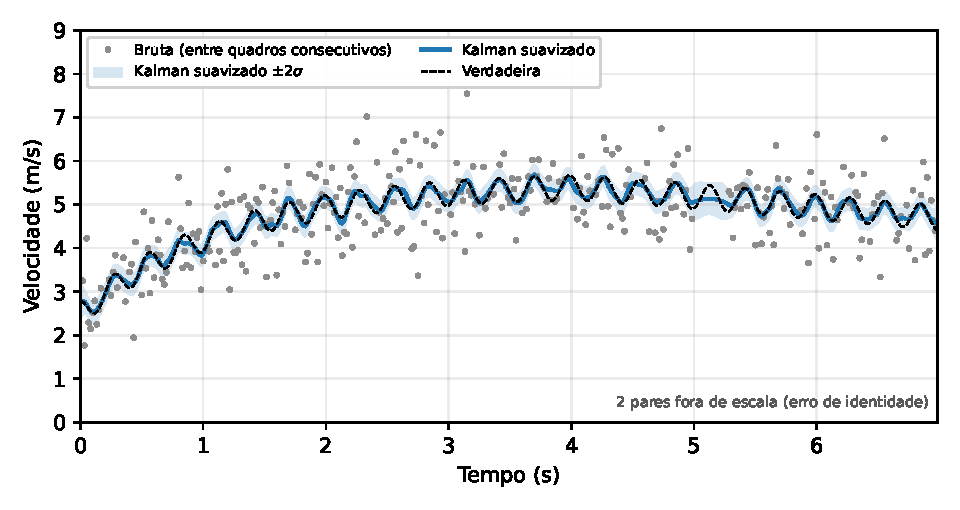
\includegraphics[width=\textwidth]{figuras/sintetico_kalman.pdf}
\fonte{Elaborado pelo autor (2026), com \texttt{src/gerar\_figuras.py}.}
\label{fig:sintetico}
\end{figure}

% NOVO
\begin{table}[H]
\centering
\small
\caption{Critérios de aceitação do teste com dados sintéticos}
\label{tab:sintetico}
\begin{tabular}{L{0.50\textwidth}L{0.40\textwidth}}
\hline
\textbf{Critério (escrito antes do teste)} & \textbf{Resultado} \\
\hline
1. O erro de identidade é rejeitado, e nenhuma outra medição & Atendido \\
2. NIS médio entre 0,7 e 1,3 & Atendido: 0,98 \\
3. Faixa de $\pm 2\sigma$ do suavizador contém a velocidade verdadeira em pelo menos 90\% dos quadros & Atendido: 100\% \\
4. Erro quadrático médio menor que 1/3 do da velocidade bruta & Atendido: 0,086 contra 0,646~m/s \\
\hline
\end{tabular}
\fonte{Elaborado pelo autor (2026).}
\end{table}
% fonte: src/validar_kalman.py

\subsection{Hipóteses Declaradas e Ajustes a Posteriori}

Antes de aplicar o filtro aos ensaios de 20~m, foram declaradas hipóteses e os critérios para considerar o filtro ruim: a velocidade média mudar além de 0,1\%, o NIS médio sair do intervalo de 0,7 a 1,3, o quadro 279 não ser rejeitado, ou o suavizador achatar as variações reais de velocidade do Ensaio C.

A versão inicial do filtro (variância de medição dada só por $\sigma_x$ e teste de inovação a 3 desvios padrão) rejeitou medições boas demais: 7 a 10 quadros no Ensaio B e 19 a 29 no Ensaio C, quando se esperava cerca de 1. Foram feitas, então, \textbf{duas revisões depois de ver os dados}, ambas declaradas como tais:
\begin{itemize}
    \item \textbf{Revisão A:} a variância de medição passou a ser estimada por máxima verossimilhança, em conjunto com $q$. O resultado foi $\kappa = 1{,}26$, isto é, $R = (1{,}26\,\sigma_x C)^2$, nos dois vídeos: a mediana dos desvios, por ser pouco sensível a valores extremos, subestima um erro que tem mais valores grandes do que a distribuição gaussiana prevê.
    \item \textbf{Revisão B:} o limite do teste de inovação passou de 3 para 5 desvios padrão. Com 3, o filtro rejeitava 5 quadros seguidos (317 a 321 do Ensaio C), que correspondem a um surto real de velocidade dentro da passada, e não a erro de detecção.
\end{itemize}
A Tabela \ref{tab:sensibilidade} mostra a sensibilidade ao limite. De 4 a 10 desvios padrão o resultado é estável, e 5 fica no meio desse intervalo.

\begin{table}[H]
\centering
\small
\caption{Sensibilidade ao limite do teste de inovação}
\label{tab:sensibilidade}
\begin{tabular}{lcccc}
\hline
\textbf{Limite} & \textbf{Rejeitados} & \textbf{Rejeitados} & \textbf{$\bar{v}_K$} & \textbf{NIS médio} \\
 & \textbf{Ensaio B} & \textbf{Ensaio C} & \textbf{Ensaio C (m/s)} & \textbf{Ensaio C} \\
\hline
3$\sigma$ (NIS $>$ 9) & 3 & 9 (inclui 317--321) & 2,7651 & 0,77 \\
4$\sigma$ (NIS $>$ 16) & 0 & 1 (quadro 279) & 2,7652 & 0,88 \\
\textbf{5$\sigma$ (NIS $>$ 25)} & \textbf{0} & \textbf{1 (quadro 279)} & \textbf{2,7651} & \textbf{1,00} \\
10$\sigma$ (NIS $>$ 100) & 0 & 1 (quadro 279) & 2,7651 & 1,00 \\
Sem teste & 0 & 0 & 2,7638 & 21,81 \\
\hline
\end{tabular}
\fonte{Elaborado pelo autor (2026).}
\end{table}
% fonte: experimentos/2026-10-07-kalman.md (seção 8); src/sensibilidade_limiar.py

Sem o teste, o quadro 279 contamina o filtro (NIS médio de 21,81). A velocidade média varia menos de 0,01\% em qualquer limite com teste.

\subsection{Resultado Final}

As Figuras \ref{fig:vel_trotando}, \ref{fig:vel_correndo} e \ref{fig:vel_variando} mostram a velocidade bruta, a curva do suavizador com faixa de $\pm 2\sigma$ e a velocidade média no trecho pela visão computacional e pelo cronômetro.

\begin{figure}[htbp]
\centering
\caption{Velocidade instantânea no Ensaio A (trote, 5~m)}
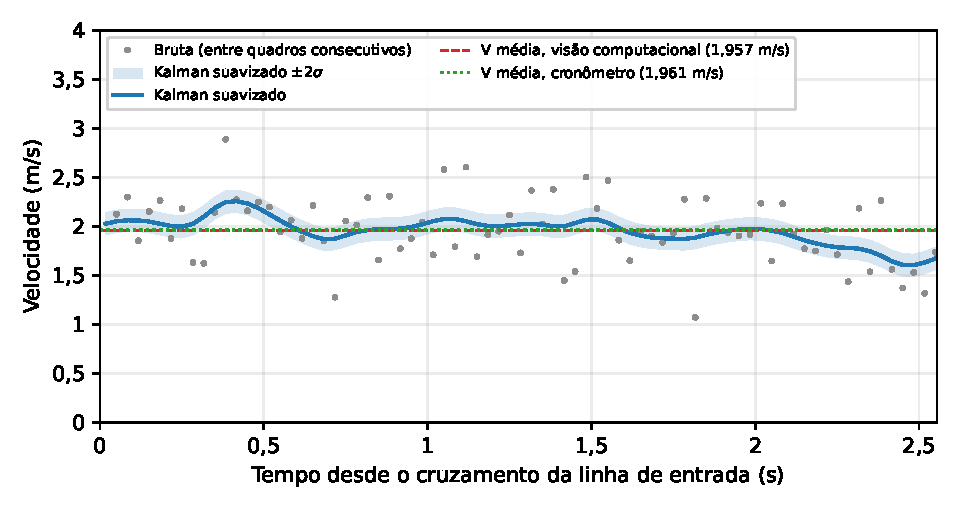
\includegraphics[width=\textwidth]{figuras/velocidade_Trotando_2.pdf}
\fonte{Elaborado pelo autor (2026), com \texttt{src/gerar\_figuras.py}.}
\label{fig:vel_trotando}
\end{figure}

\begin{figure}[htbp]
\centering
\caption{Velocidade instantânea no Ensaio B (aceleração, 20~m)}
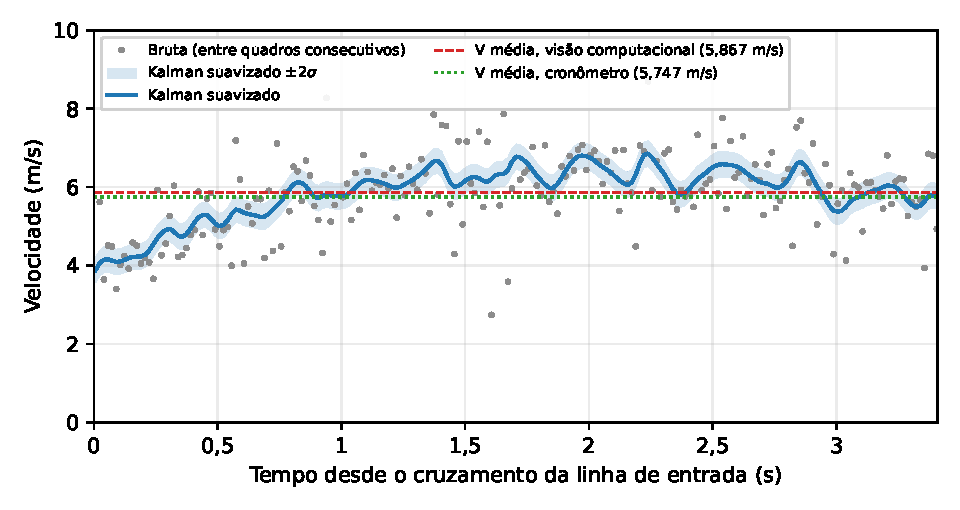
\includegraphics[width=\textwidth]{figuras/velocidade_J_Correndo.pdf}
\fonte{Elaborado pelo autor (2026), com \texttt{src/gerar\_figuras.py}.}
\label{fig:vel_correndo}
\end{figure}

\begin{figure}[htbp]
\centering
\caption{Velocidade instantânea no Ensaio C (velocidade variada, 20~m)}
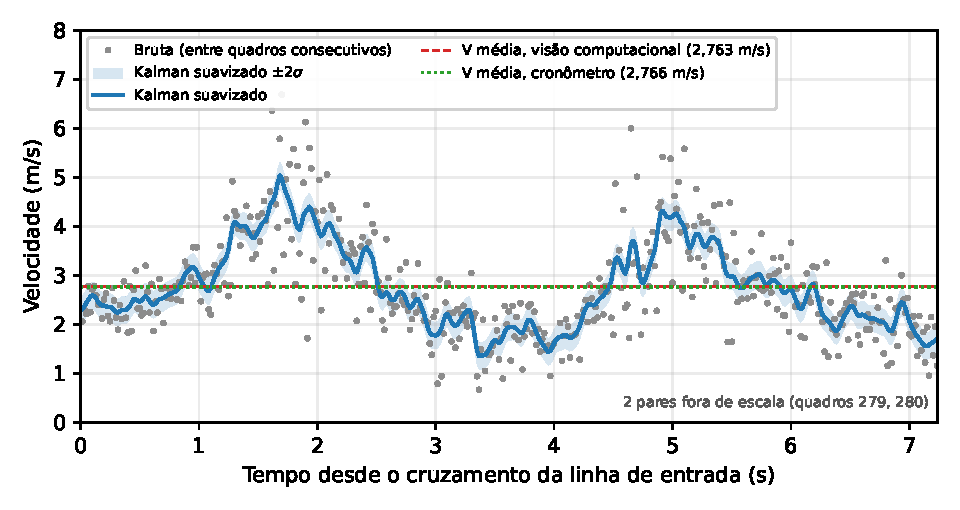
\includegraphics[width=\textwidth]{figuras/velocidade_J_Variando.pdf}
\fonte{Elaborado pelo autor (2026), com \texttt{src/gerar\_figuras.py}.}
\label{fig:vel_variando}
\end{figure}

\begin{table}[H]
\centering
\small
\caption{Resultado do filtro de Kalman (variância de medição por máxima verossimilhança, teste de inovação a 5 desvios padrão)}
\label{tab:kalman}
\begin{tabular}{L{0.36\textwidth}ccc}
\hline
 & \textbf{Ensaio A} & \textbf{Ensaio B} & \textbf{Ensaio C} \\
\hline
Ruído de medição, $\sigma_z = \sqrt{R}$ (cm) & 0,78 & 0,96 & 0,71 \\
Ruído de medição, $\sigma_z$ (pixels) & 1,29 & 0,72 & 0,53 \\
Fator $\kappa$ & 1,26 & 1,26 & 1,26 \\
Intensidade $q$ (m$^2$/s$^3$) & 0,15 & 2,75 & 2,0 \\
NIS médio & 1,03 & 1,01 & 1,00 \\
Fração do NIS acima de 3,84 & 4,8\% & 6,5\% & 5,1\% \\
Autocorrelação das inovações entre quadros consecutivos (tolerância) & $+0{,}21$ ($\pm 0{,}20$) & $+0{,}08$ ($\pm 0{,}12$) & $+0{,}11$ ($\pm 0{,}09$) \\
Quadros rejeitados & nenhum & nenhum & 279 \\
\hline
\end{tabular}
\fonte{Elaborado pelo autor (2026).}
\end{table}
% fonte: experimentos/2026-10-07-kalman.md (seção 8); experimentos/2026-10-17-trotando_2.md; diagnostico/kalman_caracterizacao.md (seções 1 e 5)

A autocorrelação das inovações passou um pouco da tolerância nos Ensaios A e C. A oscilação da passada, que o modelo de velocidade quase constante não representa, deixa a inovação de um quadro parecida com a do quadro seguinte. Também se testou um modelo que inclui a oscilação da passada como um oscilador; ele encontrou a passada (3,5~Hz no Ensaio B), mas não melhorou o ajuste aos dados de forma relevante, e o modelo de velocidade quase constante foi mantido.
% fonte: diagnostico/kalman_caracterizacao.md (seção 5); experimentos/2026-10-07-kalman.md (seção 5)

A velocidade instantânea bruta varia muito mais do que a velocidade real do corredor, e essa dispersão vem em grande parte do ruído de posição amplificado pela derivada (Seção \ref{sec:orcamento}). Nos ensaios de 20~m, medida em torno da tendência de 0,5~s, que inclui o ruído e a oscilação da passada, mas não a aceleração do corredor, a dispersão caiu cerca de 3,5 vezes com o suavizador, e as variações reais de velocidade continuam visíveis (Figura \ref{fig:vel_variando} e Tabela \ref{tab:efeito}). Qualquer suavizador reduz a dispersão; a medida de redução de erro é o teste com dados sintéticos.

% NOVO
\begin{table}[H]
\centering
\small
\caption{Efeito do suavizador sobre a velocidade instantânea}
\label{tab:efeito}
\begin{tabular}{L{0.40\textwidth}ccc}
\hline
 & \textbf{Ensaio A} & \textbf{Ensaio B} & \textbf{Ensaio C} \\
\hline
Faixa no trecho, bruta (m/s) & 1,07 a 2,89 & 2,74 a 9,50 & 0,66 a 6,69* \\
Faixa no trecho, suavizada (m/s) & 1,60 a 2,26 & 3,89 a 6,86 & 1,35 a 5,04 \\
Dispersão em torno da tendência de 0,5~s, bruta e suavizada (m/s) & --- & 0,91 e 0,26 & 0,66 e 0,24 \\
Desvio padrão médio do suavizador (m/s) & 0,057 & 0,163 & 0,134 \\
\hline
\end{tabular}

{\footnotesize Nota: * sem o par do quadro 279; --- não calculada.}
\fonte{Elaborado pelo autor (2026).}
\end{table}
% fonte: experimentos/2026-10-07-kalman.md (seções 4.2 e 8); relatório de src/analisar_cruzamentos.py (faixas); diagnostico/kalman_caracterizacao.md (seção 4)

\begin{table}[H]
\centering
\small
\caption{Resultado das hipóteses declaradas antes da aplicação aos ensaios de 20~m}
\label{tab:hipoteses}
\begin{tabular}{L{0.38\textwidth}L{0.52\textwidth}}
\hline
\textbf{Hipótese} & \textbf{Resultado} \\
\hline
1. Desvio padrão da velocidade no trecho $\le$ 0,35~m/s & \textbf{Falhou como escrita}: a métrica incluía a aceleração real do corredor. Pela métrica em torno da tendência, escolhida depois, a redução foi de cerca de 3,5 vezes. \\
2. $\bar{v}_K$ a $\le$ 0,1\% de $\bar{v}$ & Confirmada ($-0{,}10\%$ e $+0{,}06\%$), no limite no Ensaio B. \\
3. Quadro 279 rejeitado & Confirmada, sem nenhuma outra rejeição. \\
4. NIS médio entre 0,7 e 1,3 & Confirmada (1,01 e 1,00), mas só depois da revisão A. \\
\hline
\end{tabular}
\fonte{Elaborado pelo autor (2026).}
\end{table}
% fonte: experimentos/2026-10-07-kalman.md (seções 5 e 8)

\textbf{Ressalvas.} Os dois ajustes feitos depois de ver os dados (variância de medição e limite do teste) têm justificativa mecânica e sensibilidade tabelada, e foram verificados em um vídeo novo (Seção \ref{sec:resultado_trotando}), mas precisam ser confirmados em mais vídeos, sem reajuste. A intensidade $q$ é constante em cada vídeo, e surtos rápidos de velocidade dentro da passada ficam suavizados.
% fonte: experimentos/2026-10-07-kalman.md (seção 5, ressalvas honestas)

% NOVO
\subsection{Verificação em Ensaio Independente}
\label{sec:resultado_trotando}

O Ensaio A não participou da escolha do fator de $R$ nem do limite de 5 desvios padrão e serviu para verificá-los. As hipóteses foram escritas antes de rodar a análise, e o método ficou congelado: nenhum parâmetro foi mudado por causa deste vídeo (Tabela \ref{tab:hipoteses_trotando}).

\begin{table}[H]
\centering
\small
\caption{Hipóteses declaradas antes da análise do Ensaio A}
\label{tab:hipoteses_trotando}
\begin{tabular}{L{0.42\textwidth}L{0.48\textwidth}}
\hline
\textbf{Hipótese} & \textbf{Resultado} \\
\hline
1. Disponibilidade no trecho $\ge$ 90\% e cruzamentos com intervalo $\le$ 0,25~s & Confirmada: 100\%; os dois cruzamentos entre quadros consecutivos (33~ms). \\
2. NIS médio entre 0,7 e 1,3 & Confirmada: 1,03, com $\kappa = 1{,}26$, o mesmo valor dos outros dois ensaios. \\
3. Nenhuma rejeição além de erro de identidade & Confirmada: nenhum quadro rejeitado; a maior inovação aceita foi de 2,9 desvios padrão. \\
4. $\bar{v}_K$ a $\le$ 0,2\% de $\bar{v}$ & Confirmada: $+0{,}11\%$. \\
5. Centro dos ombros com ruído menor que o do centro do quadril & \textbf{Refutada}: ombros com 1,02 pixel e quadril com 0,93 pixel (Seção \ref{sec:resultado_ponto}). \\
\hline
\end{tabular}
\fonte{Elaborado pelo autor (2026).}
\end{table}
% fonte: experimentos/2026-10-17-trotando_2.md (hipóteses)

As duas escolhas do filtro feitas depois de ver os dados se mantiveram em um vídeo com metade da taxa de quadros e menor resolução: o fator de $R$ saiu de novo 1,26, o NIS médio foi 1,03 e nenhuma medição foi rejeitada. A hipótese sobre o ponto do corpo não se confirmou neste vídeo, e o resultado é discutido na Seção \ref{sec:resultado_ponto}.

% NOVO
\subsection{Ganho de Kalman e Resposta em Frequência}
\label{sec:resultado_ganho}

A Tabela \ref{tab:ganho} mostra o ganho de Kalman e a incerteza da velocidade nos três ensaios. O ganho de velocidade menor no Ensaio A acompanha o $q$ menor: em um trote de ritmo regular, a verossimilhança escolhe um modelo que espera pouca variação de velocidade de um quadro para o outro. Nos três ensaios, o desvio padrão do suavizador é cerca de metade do desvio do filtro causal.

\begin{table}[H]
\centering
\small
\caption{Ganho de Kalman e incerteza da velocidade}
\label{tab:ganho}
\begin{tabular}{L{0.46\textwidth}ccc}
\hline
 & \textbf{Ensaio A} & \textbf{Ensaio B} & \textbf{Ensaio C} \\
\hline
Ganho de posição na 2ª / 3ª medição & 1,00 / 0,84 & 1,00 / 0,84 & 1,00 / 0,84 \\
Ganho de velocidade na 2ª / 3ª medição (s$^{-1}$) & 30,0 / 15,2 & 59,6 / 30,6 & 59,8 / 30,9 \\
Ganho de posição em regime & 0,54 & 0,58 & 0,60 \\
Ganho de velocidade em regime (s$^{-1}$) & 6,2 & 14,5 & 16,2 \\
Variação típica da velocidade em um quadro, $\sqrt{q\,\Delta t}$ (m/s) & 0,07 & 0,21 & 0,18 \\
Desvio padrão médio da velocidade, filtro causal (m/s) & 0,104 & 0,295 & 0,240 \\
Desvio padrão médio da velocidade, suavizador (m/s) & 0,057 & 0,163 & 0,134 \\
\hline
\end{tabular}
\fonte{Elaborado pelo autor (2026).}
\end{table}
% fonte: diagnostico/kalman_caracterizacao.md (seções 1, 2 e 4)

A Tabela \ref{tab:inovacao} mostra as grandezas do teste de inovação usadas na escolha do limite (Seção \ref{sec:kalman}).

\begin{table}[H]
\centering
\small
\caption{Teste de inovação nos três ensaios}
\label{tab:inovacao}
\begin{tabular}{L{0.42\textwidth}L{0.14\textwidth}L{0.14\textwidth}L{0.18\textwidth}}
\hline
 & \textbf{Ensaio A} & \textbf{Ensaio B} & \textbf{Ensaio C} \\
\hline
Desvio padrão esperado da inovação, $\sqrt{S_k}$ (mediana) & 1,15~cm & 1,48~cm & 1,12~cm \\
Maior inovação aceita & 2,9$\sigma$ (quadro 70) & 3,9$\sigma$ (quadro 387) & 4,2$\sigma$ (quadro 317) \\
Inovações aceitas acima de 3$\sigma$ / 4$\sigma$ & 0 / 0 & 4 / 0 & 8 / 1 \\
Medição rejeitada & nenhuma & nenhuma & quadro 279: 8,50~m, ou 757$\sigma$ \\
Rejeições esperadas a 3$\sigma$ / 5$\sigma$ se o erro fosse gaussiano & 0,29 / 0,0001 & 0,71 / 0,0002 & 1,33 / 0,0003 \\
\hline
\end{tabular}
\fonte{Elaborado pelo autor (2026).}
\end{table}
% fonte: diagnostico/kalman_caracterizacao.md (seção 3)

Outra forma de ver o efeito do ganho é a resposta em frequência (Tabela \ref{tab:frequencia}). Aplica-se ao filtro, com o $q$ e o $R$ de cada ensaio, uma oscilação senoidal de posição de amplitude conhecida, sem ruído, e mede-se que fração da oscilação de velocidade correspondente aparece na estimativa. Nos ensaios de 20~m, o suavizador funciona como um filtro passa-baixas sem atraso, com frequência de corte (ganho de 0,707) de 4,7 e 5,1~Hz: mantém 88\% e 91\% da oscilação da passada a 3,5~Hz e remove mais de 97\% do que está acima de 15~Hz. O filtro causal corta um pouco acima (5,9 e 6,4~Hz), mas atrasa a estimativa em cerca de 30~ms. No Ensaio A, com $q$ menor, o corte do suavizador cai para 2,2~Hz, e ele mantém só 24\% da oscilação a 3,5~Hz. Ao contrário do corte de 3~Hz usado no laser, a frequência de corte aqui não é escolhida a priori: ela resulta da razão entre $q$ e $R$ estimados nos próprios dados.
% fonte: diagnostico/kalman_caracterizacao.md (seção 6)

\begin{table}[H]
\centering
\small
\caption{Resposta em frequência na velocidade: fração da oscilação que aparece na estimativa}
\label{tab:frequencia}
\footnotesize
\setlength{\tabcolsep}{4pt}
\begin{tabular}{lcccccc}
\hline
 & \multicolumn{2}{c}{\textbf{Ensaio A}} & \multicolumn{2}{c}{\textbf{Ensaio B}} & \multicolumn{2}{c}{\textbf{Ensaio C}} \\
\textbf{Frequência (Hz)} & Filtro & Suavizador & Filtro & Suavizador & Filtro & Suavizador \\
\hline
2 & 0,87 & 0,75 & 0,99 & 0,99 & 1,00 & 0,99 \\
3,5 & 0,50 & 0,24 & 0,95 & 0,88 & 0,96 & 0,91 \\
5 & 0,28 & 0,07 & 0,81 & 0,65 & 0,85 & 0,71 \\
10 & 0,08 & 0,00 & 0,34 & 0,10 & 0,38 & 0,13 \\
15 & --- & --- & 0,17 & 0,02 & 0,19 & 0,03 \\
Corte (ganho 0,707), Hz & 2,7 & 2,2 & 5,9 & 4,7 & 6,4 & 5,1 \\
Atraso de 0,5 a 3,5~Hz (ms) & 72 a 81 & 0 & 32 a 35 & 0 & 29 a 32 & 0 \\
\hline
\end{tabular}

{\footnotesize Nota: 15~Hz é a metade da taxa de quadros do Ensaio A e não é avaliada nele.}
\fonte{Elaborado pelo autor (2026).}
\end{table}
% fonte: diagnostico/kalman_caracterizacao.md (seção 6)

% ----------------------------------------------------------
% SEÇÃO 4.4 - ORÇAMENTO DE ERRO
% ----------------------------------------------------------
\section{Orçamento de Erro}
\label{sec:orcamento}

Esta seção reúne as contribuições do processamento para a incerteza da velocidade média no trecho e o efeito da taxa de quadros, calculados a partir dos três ensaios. Ela descreve as componentes de incerteza do processamento, e não a exatidão, porque a referência dos ensaios é o cronômetro.

\begin{table}[H]
\centering
\small
\caption{Contribuições do processamento para a incerteza da velocidade média}
\label{tab:orcamento}
\begin{tabular}{L{0.40\textwidth}L{0.36\textwidth}L{0.12\textwidth}}
\hline
\textbf{Componente} & \textbf{Efeito: Ensaio A / B / C} & \textbf{Situação} \\
\hline
Ruído do ponto medido, no tempo dos cruzamentos (com interpolação) & 0,23\% / 0,11\% / 0,06\% & medido \\
Base de tempo (resíduo dos carimbos) & abaixo de 0,001\% nos três & medido \\
Calibração por cliques & $\approx$ 0,09\% / 0,07\% / 0,07\% & estimado \\
\hline
\end{tabular}
\fonte{Elaborado pelo autor (2026).}
\end{table}
% fonte: diagnostico/orcamento_erro.md (seção 1); src/orcamento_erro.py (seções 0 e 1)

A componente da calibração supõe que cada clique erra até meia resolução de clique, em cada uma das duas marcações: 0,5 pixel no Ensaio A e 0,74 pixel nos de 20~m, em que a janela de calibração é reduzida para caber na tela e cada pixel da tela vale 1,48 pixel do vídeo. Com 1504 pixels entre as marcações, isso dá $\sqrt{2} \times 0{,}74 / 1504 \approx 0{,}07\%$.
% fonte: calibracao/*.json (resolucao_clique_px); src/orcamento_erro.py (seção 0)

\subsection{Efeito da Taxa de Quadros}
Sem interpolação, o tempo de cada linha teria erro de até um quadro, 33,3~ms a 30 quadros por segundo e 16,7~ms a 60, e o desvio da velocidade média chegaria a 0,53\% no Ensaio A. Com a interpolação, o limite passa a ser o ruído do ponto medido: o tempo de cruzamento erra cerca de $\sigma_z / v$, em que $\sigma_z$ é o desvio padrão do ruído de medição (Equação \ref{eq:kalman_r}) e $v$ a velocidade do corredor na linha, de 4,5 a 9,5 vezes menos que o intervalo entre quadros. Daí vem a primeira linha da Tabela \ref{tab:orcamento}.
% fonte: diagnostico/orcamento_erro.md (seção 2)

Para verificar o efeito do número de quadros, foram removidos quadros do vídeo, em todas as fases possíveis (Tabela \ref{tab:fps}).

\begin{table}[H]
\centering
\small
\caption{Maior desvio da velocidade média em relação ao resultado na taxa original}
\label{tab:fps}
\footnotesize
\begin{tabular}{lccc}
\hline
\textbf{Ensaio (taxa original)} & \textbf{Taxa (fps)} & \textbf{Com interpolação} & \textbf{Sem interpolação} \\
\hline
Ensaios B / C (60 fps) & 30 & 0,08\% / 0,07\% & 0,69\% / 0,40\% \\
 & 20 & 0,15\% / 0,10\% & 1,17\% / 0,17\% \\
 & 15 & 0,26\% / 0,08\% & 1,64\% / 0,52\% \\
 & 10 & 0,31\% / 0,10\% & 2,58\% / 0,86\% \\
Ensaio A (30 fps) & 15 & 0,01\% & 1,73\% \\
 & 10 & 0,11\% & 2,20\% \\
 & 7,5 & 0,15\% & 4,19\% \\
 & 5 & 0,47\% & 6,46\% \\
\hline
\end{tabular}
\fonte{Elaborado pelo autor (2026).}
\end{table}
% fonte: diagnostico/orcamento_erro.md (seção 2)

Para a velocidade média, a interpolação torna a taxa de quadros pouco relevante: nos ensaios de 20~m, 10 quadros por segundo com interpolação têm desvio menor que 30 quadros por segundo sem ela, e no Ensaio A, 7,5 quadros por segundo com interpolação desviam 0,15\%, contra 1,73\% a 15 quadros por segundo sem interpolação. O teste simula taxas menores removendo quadros do mesmo vídeo.

A taxa de quadros pesa na velocidade instantânea. A derivada entre dois quadros consecutivos tem erro de cerca de $\sqrt{2}\,\sigma_z f$ (primeira linha da Tabela \ref{tab:janela}); em janelas maiores, o erro da velocidade média cai. O desvio padrão do suavizador muda pouco quando a taxa de quadros cai (últimas linhas da mesma tabela).
% fonte: diagnostico/orcamento_erro.md (seção 2)

\begin{table}[H]
\centering
\caption{Erro padrão da velocidade (m/s): bruta, em janelas de duração $T$, e do suavizador em taxas reduzidas}
\label{tab:janela}
\small
\begin{tabular}{lccc}
\hline
 & \textbf{Ensaio A} & \textbf{Ensaio B} & \textbf{Ensaio C} \\
\hline
1 quadro (bruta, valor teórico) & 0,33 & 0,82 & 0,60 \\
Janela de 0,10 s & 0,09 & 0,11 & 0,08 \\
Janela de 0,286 s (um ciclo de 3,5 Hz) & 0,04 & 0,04 & 0,03 \\
\hline
Suavizador, taxa original & 0,057 & 0,163 & 0,134 \\
Suavizador, metade da taxa & 0,052 & 0,170 & 0,139 \\
Suavizador, um quarto da taxa & 0,048 & 0,196 & 0,148 \\
\hline
\end{tabular}
\fonte{Elaborado pelo autor (2026).}
\end{table}
% fonte: diagnostico/orcamento_erro.md (seção 2)

\subsection{Escolha do Ponto de Medição}
\label{sec:resultado_ponto}
Com as mesmas linhas e o mesmo critério de confiança, a velocidade média e o ruído de posição foram calculados com outros pontos do corpo (Tabela \ref{tab:pontos}). A disponibilidade no trecho foi de 100\% para todos os pontos nos três ensaios.

\begin{table}[H]
\centering
\small
\caption{Ruído de posição e diferença da velocidade média contra o centro dos ombros}
\label{tab:pontos}
\begin{tabular}{L{0.26\textwidth}L{0.28\textwidth}L{0.36\textwidth}}
\hline
\textbf{Ponto} & \textbf{Ruído $\sigma_x$ (px): Ensaio A / B / C} & \textbf{Diferença de $\bar{v}$: Ensaio A / B / C} \\
\hline
\textbf{Centro dos ombros} & \textbf{1,02 / 0,58 / 0,42} & --- \\
Ombro esquerdo & 1,02 / 0,95 / 0,56 & $+4{,}08\%$ / $+0{,}74\%$ / $+1{,}44\%$ \\
Ombro direito & 1,78 / 1,50 / 0,89 & $-4{,}57\%$ / $-1{,}08\%$ / $-1{,}45\%$ \\
Centro do quadril & 0,93 / 0,81 / 0,58 & $+0{,}07\%$ / $+1{,}97\%$ / $+0{,}72\%$ \\
Nariz & 0,63 / 0,59 / 0,58 & $+1{,}26\%$ / $-1{,}11\%$ / $+0{,}11\%$ \\
Centro da caixa delimitadora & 1,92 / 1,34 / 0,68 & $+1{,}51\%$ / $+2{,}44\%$ / $+1{,}53\%$ \\
\hline
\end{tabular}
\fonte{Elaborado pelo autor (2026).}
\end{table}
% fonte: diagnostico/orcamento_erro.md (seção 3)

Nos dois ensaios de 20~m, o centro dos ombros teve o menor ruído entre os pontos testados; no Ensaio B, empatou com o nariz. O centro do quadril teve cerca de 40\% mais ruído, e o centro da caixa delimitadora, de 1,6 a 2,3 vezes mais, o que confirma a razão inicial para não usar a caixa: ela oscila com os braços e as pernas. Contra o cronômetro, a velocidade pelos ombros ficou mais perto que a do quadril nos dois ensaios, mas a incerteza do cronômetro não permite ordenar os pontos pela exatidão; o critério que decide é o ruído.
% fonte: diagnostico/orcamento_erro.md (seção 3); cálculo: 0,81 / 0,58 e 0,58 / 0,42

No Ensaio A, em trote a 30 quadros por segundo, o centro do quadril teve ruído 9\% menor que o dos ombros, e o nariz foi o ponto de menor ruído. Uma hipótese, não testada, é que, com quadros 33~ms afastados, a segunda diferença capta mais a oscilação horizontal real dos ombros, causada pela rotação do tronco e pelo balanço dos braços. Com três ensaios, o centro dos ombros tem o menor ruído em dois.
% fonte: diagnostico/orcamento_erro.md (seção 3); experimentos/2026-10-17-trotando_2.md (hipótese 5)

Cada ombro isolado dá velocidade média diferente da do centro, em sentidos opostos. Como o corredor passa da direita para a esquerda, o ombro esquerdo fica mais perto da câmera e parece andar mais pixels, e o direito, mais longe, parece andar menos; o efeito é maior no Ensaio A, com a câmera a 6~m, do que nos de 20~m, com a câmera a 21~m. O centro dos ombros, entre os dois, cancela esse efeito. A comparação entre pontos deve ser repetida nos vídeos da sessão com fotocélulas, em que a exatidão de cada ponto pode ser medida.

% NOVO
% ----------------------------------------------------------
% SEÇÃO 4.5 - COMPARAÇÃO COM AS FOTOCÉLULAS
% ----------------------------------------------------------
\section{Comparação com as Fotocélulas}
\label{sec:resultado_fotocelula}

Esta seção recebe os resultados da sessão com fotocélulas (Seção \ref{sec:sessao_fotocelulas}) [VALOR A MEDIR].

\begin{table}[H]
\centering
\small
\caption{Sistema de visão contra fotocélulas}
\label{tab:fotocelula}
\begin{tabular}{L{0.40\textwidth}L{0.22\textwidth}L{0.22\textwidth}}
\hline
 & \textbf{$\bar{v}$, sem filtro} & \textbf{$\bar{v}_K$, com filtro} \\
\hline
Número de passagens & \multicolumn{2}{c}{[VALOR A MEDIR]} \\
Faixa de velocidades de referência (m/s) & \multicolumn{2}{c}{[VALOR A MEDIR]} \\
Diferença média para a fotocélula & [VALOR A MEDIR] & [VALOR A MEDIR] \\
Desvio padrão das diferenças (erro típico) & [VALOR A MEDIR] & [VALOR A MEDIR] \\
Menor mudança relevante & \multicolumn{2}{c}{$\approx 1\%$} \\
Erro típico $\le$ menor mudança relevante? & [VALOR A MEDIR] & [VALOR A MEDIR] \\
\hline
\end{tabular}
\fonte{Elaborado pelo autor (2026).}
\end{table}

% ----------------------------------------------------------
% SEÇÃO 4.6 - DISCUSSÃO
% ----------------------------------------------------------
\section{Discussão}

Os resultados sustentam as seguintes afirmações, dentro dos limites de três ensaios preliminares e um corredor:
\begin{itemize}
    \item Com o arquivo original e a resolução nativa, os trechos de 5 e de 20~m foram cobertos em todos os quadros, e os cruzamentos foram interpolados entre quadros consecutivos, nos três ensaios.
    \item A contribuição do ruído de posição para a incerteza da velocidade média fica entre 0,06\% e 0,23\%, com interpolação, e depende pouco da taxa de quadros.
    \item Em dados sintéticos, o suavizador reduziu cerca de 7,5 vezes o erro da velocidade instantânea. Nos ensaios, reduziu a dispersão sem alterar a velocidade média de forma relevante, manteve as variações reais de velocidade e rejeitou o único erro de identidade. As escolhas do filtro feitas depois de ver os dados se mantiveram no Ensaio A.
    \item O maior efeito identificado é a escolha do ponto do corpo: cada ombro isolado muda a velocidade média em até 4,6\%, e o centro dos ombros cancela esse efeito. O centro dos ombros teve o menor ruído nos dois ensaios de 20~m, mas não no trote.
\end{itemize}
% fonte: resultados/ensaios.csv; diagnostico/orcamento_erro.md; diagnostico/kalman_caracterizacao.md; experimentos/2026-10-07-kalman.md; src/validar_kalman.py

Os resultados não sustentam afirmações sobre exatidão. O cronômetro manual tem incerteza maior que a do processamento, e por isso as diferenças para ele não permitem concluir se há viés. O critério de que o erro típico seja menor ou igual à menor mudança relevante (Seção \ref{sec:criterios}) depende da comparação com as fotocélulas (Seção \ref{sec:resultado_fotocelula}) [VALOR A MEDIR].

Outras limitações do processamento: a regra de seleção da pessoa pela maior caixa é frágil quando há outras pessoas ou objetos na cena, embora o filtro rejeite o erro resultante; a intensidade $q$ é constante em cada vídeo, e surtos rápidos de velocidade dentro da passada ficam suavizados; e a base de tempo foi verificada pelos carimbos lidos com OpenCV, não pelo contêiner do vídeo.
% fonte: diagnostico/orcamento_erro.md (seções 4 e 5); README.md (pendências)

% ----------------------------------------------------------
% CAPÍTULO 5 - CONCLUSÃO
% ----------------------------------------------------------
\chapter{CONCLUSÃO}

\section{Considerações Finais}
Este trabalho desenvolveu um sistema que estima a velocidade de corrida a partir do vídeo de uma câmera fixa, com uma rede YOLO de estimação de pose, calibração por duas marcações no solo e filtro e suavizador de Kalman, processado \textit{offline} em um computador pessoal, sem placa de vídeo. Em três ensaios preliminares, com duas montagens (5 e 20~m), duas taxas de quadros (30 e 60 por segundo) e duas resoluções, os objetivos específicos tiveram os seguintes resultados:
\begin{itemize}
    \item o processamento \textit{offline} com a rede YOLO de pose localizou o atleta em todos os quadros do trecho, nos três ensaios;
    \item a conversão de pixels para metros pelas duas marcações no solo contribui com menos de 0,1\% para a incerteza da velocidade média;
    \item a velocidade média no trecho foi calculada pela interpolação dos cruzamentos, sem e com o filtro, com diferença de até 0,11\% entre as duas; a velocidade instantânea, pelo filtro e pelo suavizador de Kalman, que em dados sintéticos reduziram o erro de 0,646 para 0,086~m/s e nos ensaios rejeitaram um erro de identidade do detector sem descartar medições boas;
    \item a contribuição do ruído de posição para a incerteza da velocidade média ficou entre 0,06\% e 0,23\%; a comparação com as fotocélulas [VALOR A MEDIR].
\end{itemize}
% fonte: resultados/ensaios.csv; diagnostico/orcamento_erro.md; experimentos/2026-10-07-kalman.md; experimentos/2026-10-17-trotando_2.md; src/validar_kalman.py

No uso que motivou este trabalho, o acompanhamento de atletas ao longo do tempo, inclusive no retorno após uma lesão, o sistema é útil se o seu erro típico for menor ou igual à menor mudança relevante, de cerca de 1\% (Seção \ref{sec:criterios}). As contribuições do processamento avaliadas aqui ficam bem abaixo desse valor; a comparação com as fotocélulas dirá se o sistema como um todo atinge o critério [VALOR A MEDIR].

\section{Limitações do Trabalho}
\begin{itemize}
    \item Três ensaios preliminares, com um único corredor, e referência por cronômetro manual, de incerteza maior que a do processamento.
    \item A regra de seleção da pessoa pela maior caixa delimitadora é frágil na presença de outras pessoas ou objetos.
    \item A intensidade $q$ do filtro é constante em cada vídeo.
    \item O fator de $R$ e o limite do teste de inovação foram escolhidos depois de ver os dados; foram verificados em um único vídeo novo.
    \item Apenas o modelo de menor tamanho (\texttt{yolo26n-pose}) foi avaliado.
    \item O centro dos ombros teve o menor ruído em dois dos três ensaios; no trote, o quadril teve menos ruído.
    \item A base de tempo foi verificada pelos carimbos lidos com OpenCV, e não pelo contêiner do vídeo.
\end{itemize}

\section{Trabalhos Futuros}
\label{sec:trabalhos_futuros}
\begin{itemize}
    \item Selecionar o atleta pela continuidade da trajetória, e não pela maior caixa delimitadora.
    \item Avaliar modelos de pose maiores, medindo o efeito sobre o ruído do ponto medido e sobre a disponibilidade.
    \item Usar um modelo de filtro com intensidade $q$ adaptativa, que acompanhe surtos rápidos de velocidade.
    \item Repetir a comparação entre pontos do corpo nos vídeos da sessão com fotocélulas, em que a exatidão de cada ponto pode ser medida.
    \item Medir \textit{online}: o orçamento de erro mostra que a interpolação torna a velocidade média no trecho pouco sensível à taxa de quadros, e o filtro causal já existe; o limite atual é o tempo de inferência em CPU, de 112 a 292~ms por quadro.
\end{itemize}
% PENDENTE: tentativa de sistema embarcado (fatos a fornecer pelo autor: equipamento, versão do YOLO, quadros por segundo obtidos e por que parou).

% ----------------------------------------------------------
% ELEMENTOS PÓS-TEXTUAIS
% ----------------------------------------------------------
\postextual

% --- Referências Bibliográficas ---
\bibliography{referencias} % Criação automática das referências a partir do .bib

% NOVO
% --- Apêndices ---
\begin{apendicesenv}
\partapendices

\chapter{Repositório e Reprodução dos Resultados}
\label{ap:repositorio}

O código, as calibrações, os pontos-chave extraídos pela rede neural e os registros dos ensaios e dos experimentos estão no repositório do trabalho \cite{santos2026repositorio}. Os vídeos não são públicos, porque mostram pessoas; os arquivos de pontos-chave permitem reproduzir todos os resultados a partir da etapa de análise, sem rodar a rede neural. Os programas rodam a partir da pasta do repositório, no ambiente Python com as versões da Tabela \ref{tab:versoes}.

\begin{table}[H]
\centering
\small
\caption{Versões do ambiente de software}
\label{tab:versoes}
\begin{tabular}{ll}
\hline
\textbf{Componente} & \textbf{Versão} \\
\hline
Python & 3.14.7 \\
\texttt{opencv-python} & 5.0.0.93 \\
\texttt{numpy} & 2.5.3 \\
\texttt{torch} (CPU) / \texttt{torchvision} & 2.14.1 / 0.29.1 \\
\texttt{ultralytics} & 8.4.174 \\
\texttt{pillow} (só exibição) & 12.3.0 \\
Pesos \texttt{yolo26n-pose.pt} (MD5) & \texttt{af743a72087d8101c1025b9165056f79} \\
\hline
\end{tabular}
\fonte{Elaborado pelo autor (2026).}
\end{table}
% fonte: requirements.txt; resultados/keypoints/*_imgsz*.json (versoes e md5 dos pesos)

\begin{table}[H]
\centering
\small
\caption{Programa que gera cada tabela e figura}
\label{tab:reproducao}
\begin{tabular}{L{0.30\textwidth}L{0.60\textwidth}}
\hline
\textbf{Tabela ou figura} & \textbf{Programa} \\
\hline
Tabelas \ref{tab:imgsz}, \ref{tab:ensaios} e \ref{tab:kalman} & \texttt{src/analisar\_cruzamentos.py}, com o CSV de pontos-chave, a calibração e o tempo do cronômetro de cada ensaio \\
Tabela \ref{tab:sintetico} e Figura \ref{fig:sintetico} & \texttt{src/validar\_kalman.py} e \texttt{src/gerar\_figuras.py} \\
Tabela \ref{tab:sensibilidade} & \texttt{src/sensibilidade\_limiar.py} \\
Tabelas \ref{tab:ganho}, \ref{tab:inovacao} e \ref{tab:frequencia} & \texttt{src/caracterizar\_kalman.py} \\
Tabelas \ref{tab:orcamento}, \ref{tab:fps}, \ref{tab:janela} e \ref{tab:pontos} & \texttt{src/orcamento\_erro.py} \\
Figuras \ref{fig:vel_trotando}, \ref{fig:vel_correndo} e \ref{fig:vel_variando} & \texttt{src/gerar\_figuras.py} \\
Figura \ref{fig:tela_variando} & \texttt{src/visualizar\_medicao.py -{}-video J\_Variando -{}-salvar-quadro} \\
\hline
\end{tabular}
\fonte{Elaborado pelo autor (2026).}
\end{table}

As hipóteses de cada experimento, escritas antes de rodá-lo, e os resultados de cada revisão ficam nos registros da pasta \texttt{experimentos}; o registro de todos os ensaios, inclusive os ruins, fica em \texttt{resultados/ensaios.csv}.

\end{apendicesenv}

\end{document}
